\documentclass{memoir}
\usepackage{notestemplate}
\usetikzlibrary{matrix,arrows.meta}

\logo{~/LibreMath/Auxiliary Resources/resources/png/logo.png}
\institute{Rice University}
%\faculty{Faculty of Whatever Sciences}
\department{Department of Mathematics}
\title{Introduction to UFDs, Modules, Finite Fields, and Galois Theory}
\subtitle{Based on MATH 357 at Rice University}
\author{\textit{Author}\\ Gabriel \textsc{Gress}}
%\supervisor{Linus \textsc{Torvalds}}
%\context{Well, I was bored...}
\date{\today}

%\makeindex

\begin{document}

\maketitle

\tableofcontents

\setcounter{chapter}{-1}

\chapter{Preamble}
\label{cha:preamble}
\documentclass{memoir}
\usepackage{notestemplate}

%\logo{./resources/pdf/logo.pdf}
%\institute{Rice University}
%\faculty{Faculty of Whatever Sciences}
%\department{Department of Mathematics}
%\title{Class Notes}
%\subtitle{Based on MATH xxx}
%\author{\textit{Author}\\Gabriel \textsc{Gress}}
%\supervisor{Linus \textsc{Torvalds}}
%\context{Well, I was bored...}
%\date{\today}

\begin{document}

% \maketitle

% Notes take on 01/25/21

\chapter{Introduction}
\label{cha:introduction}

These notes covers modules, unital and commutative rings, and fields.\\

The lecture notes are based off two main sources. The overall outline and the major statements of theorems and definitions are based off lecture notes from Dr.\@ Chelsea Walton during the Spring 2021 teaching of Rice's course MATH 357 -- \textit{Abstract Algebra II}. These notes are supplemented by exercises from Dummitt and Foote's \textit{Abstract Algebra}, and some of the basic ring material is based on Goodman's \textit{Algebra: Abstract and Concrete}. Finally, the applications of Galois theory are based on a section from Hungerford's \textit{Algebra}.

\end{document}


\documentclass{memoir}
\usepackage{notestemplate}

%\logo{./resources/pdf/logo.pdf}
%\institute{Rice University}
%\faculty{Faculty of Whatever Sciences}
%\department{Department of Mathematics}
%\title{Class Notes}
%\subtitle{Based on MATH xxx}
%\author{\textit{Author}\\Gabriel \textsc{Gress}}
%\supervisor{Linus \textsc{Torvalds}}
%\context{Well, I was bored...}
%\date{\today}

\begin{document}

% \maketitle

% Notes taken on 01/25/21

\chapter{Modules}
\label{cha:modules}

\section{Ring Review}
\label{sec:ring_review}



Recall the definition of a ring.

\begin{defn}[Ring]
	A \textbf{ring} is a nonempty set \(R\) with two operations: addition and multiplication, which has the properties
	\begin{itemize}
		\item \(R^{+}\) is an abelian group
		\item \(R^{\times }\) is a semigroup
		\item \(\times \) distributes over \(+\) :
			\begin{align*}
				a(b+c) = ab+ac \quad (b+c)a = ba+ca
			\end{align*}
	\end{itemize}
\end{defn}

\begin{defn}[Types of Rings]
	A ring \(R\) is \textbf{commutative} if \(\times \) is commutative. Furthermore, we say a ring is \textbf{unital} if there exists an element \(1_R \in R\) so that \(1_R a = a_{1_R} = a\) for all \(a \in R\).\\

The ring \(R\) is \textbf{(in)finite} if it is (in)finite as a set.\\

A \textbf{subring} of \(R\) is an additive subgroup \(S\) of \(R\) that is closed under the multiplication of \(R\). Furthermore, if it contains \(1_R\) then it is a \textbf{unital subring}.\\

A \textbf{unit} of \(R\) is an element \(a \in R\) that has a multiplicative inverse, i.e. \(\exists b \in R\) so that \(ab = ba = 1_R\). The set of units of \(R\) is sometimes denoted by \(R^{\times }\).
\end{defn}

In order to better classify commutative rings, we introduce a few more terminology.

\begin{defn}[Irreducibles and Primes]
	We say that \(r \in R\) is \textbf{irreducible} if 
	\begin{align*}
		r = ab \implies a \text{ or }b \text{ is a unit}.
	\end{align*}
	We impose a stronger condition that \(r \in R\) is \textbf{prime} if 
	\begin{align*}
		r \mid ab \implies r\mid a \text{ or }r \mid b.
	\end{align*}

\end{defn}
Note that every prime is irreducible, but not vice versa.\\

\begin{figure}[ht]
    \centering
     \def\svgwidth{1\linewidth}
     \input{./figures/hierarchy-of-commutative-rings.pdf_tex}
    \caption{Hierarchy of Commutative Rings}
    \label{fig:hierarchy-of-commutative-rings}
\end{figure}

\end{document}


\section{Rings with Divison Structures}
\label{sec:rings_with_divison_structures}

\documentclass{memoir}
\usepackage{notestemplate}

%\logo{./resources/pdf/logo.pdf}
%\institute{Rice University}
%\faculty{Faculty of Whatever Sciences}
%\department{Department of Mathematics}
%\title{Class Notes}
%\subtitle{Based on MATH xxx}
%\author{\textit{Author}\\Gabriel \textsc{Gress}}
%\supervisor{Linus \textsc{Torvalds}}
%\context{Well, I was bored...}
%\date{\today}

\begin{document}

% \maketitle

% Notes taken on 01/27/21

\begin{defn}[Norm of Integral Domain]
	Let \(R\) be an integral domain. Any function \(N:R\to \Z^{+}\cup \left\{ 0 \right\} \) with \(N(0)\) is called a \textbf{norm} on the integral domain \(R\). If \(N(a) > 0\) for \(a\neq 0\) then \(N\) is a \textbf{positive norm}
\end{defn}
This is a pretty loose construction, and an integral domain can have many norms on it.\\

\begin{defn}[Euclidean Function]
	An integral domain \(R\) is a \textbf{Euclidean Domain} if there exists a norm called the \textbf{Euclidean function} \(N:R\setminus\left\{ 0 \right\} \to \N\) that satisfies \(\forall a,b \in R\setminus \left\{ 0 \right\} \):
	\begin{align*}
		N(ab) \geq \textrm{max}\left\{ N(a),N(b) \right\}\\
		\exists q,r \in R \text{ such that }a = qb + r \text{ and }\left[ r = 0 \text{ or }N(r)<N(b) \right] 
	\end{align*}
	We call the element \(q\) the \textbf{quotient} and the element \(r\) the  \textbf{remainder}.
\end{defn}
The existence of a Euclidean function is integral to constructing a Euclidean algorithm to perform division of elements \(a,b \in R\). We can perform successive divisions to get
\begin{align*}
	a = q_0b + r_0\\
	b = q_1r_0 + r_1\\
	r_0 = q_2r_1 + r_2\\
	\vdots\\
	r_{n-1}= q_nr_{n-1}+r_n\\
	r_{n-1} = q_{n+1}r_n
\end{align*}
where \(r_n\) is the last nonzero remainder. This \(r_n\) always exists as the norms form a decreasing sequence of nonnegative integers. However, these elements are not necessarily unique.

\begin{prop}
	Every ideal in a Euclidean Domain is principal. That is, if \(I\triangleleft R\) is a nontrivial ideal in \(R\), then \(I = (d)\) for some nonzero element of \(I\) with minimum norm.
\end{prop}
This also makes it convenient to show an integral domain is not a Euclidean Domain by simply finding a non-principal ideal. Moreover, it motivates the notion of greatest common divisors from \(\Z\) into comumutative rings.

\begin{defn}[Greatest Common Divisor]
	Let \(R\) be a commutative ring and let \(a,b \in R\) with \(b\neq 0\). Then \(a\) is said to be a \textbf{multiple} of \(b\) if there exists an element \(x \in R\) with \(a=bx\). In this case, we say \(b\) \textbf{divides} \(a\) (or is a \textbf{divisor} of \(a \)) written \(b\mid a\).\\

	A \textbf{greatest common divisor} of \(a,b\) is a nonzero element \(d\) such that
	\begin{align*}
		d \mid a, \; d \mid b \\
		d'\mid a \; d'\mid b \implies d'\mid d
	\end{align*}
	We will denote a greatest common divisor by \(\textrm{gcd}(a,b)\), or sometimes simply \((a,b)\) if it is clear from context.\\

	If \(gcd(a,b) = 1_R\), then we say that \(a\) and \(b\) are \textbf{relatively prime}.
\end{defn}
We can easily extend this to finite sequences of elements \((a_1,a_2,\ldots,a_n)\).\\

Recall that in a ring \(b\mid a \iff a \in (b) \iff (a) \subset (b)\). Hence, we can discuss greatest common factors in terms of ideals. That is, if \(I = (a,b)\) is the ideal of \(R\) generated by \(a,b\), then \(d = \textrm{gcd}(a,b)\) if \(I\subset (d)\) and if \(I\subset (d') \implies (d)\subset (d')\). Thus, it is the unique smallest principal ideal containing \(a\) and \(b\). However, it may not exist in all rings.

\begin{prop}[Sufficient Conditions for Existence]
	If \(a,b \in R\) are nonzero elements in a commutative ring such that \(I = (a,b) = (d)\), then \(d\) is the greatest common divisor of \(a,b\).
\end{prop}
Obviously this is a sufficient and not a necessary condition. But it also clarifies why \((a,b)\) is used both for ideals and greatest common divisors. Any integral domain that satisfies the above condition for all ideals of two elements is called a \textbf{Bezout Domain}.

\begin{prop}
	Let \(R\) be an integral domain. If two elements \(d,d' \in R\) generate the same principal ideal, i.e. \((d) = (d')\), then \(d' = ud\) for some unit \(u \in R\). In particular, this tells us that greatest common divisors are unique up to units.
\end{prop}

\begin{thm}
	Let \(R\) be a Euclidean Domain and let \(a,b \in R\) be nonzero. Let \(d = r_n\) be the last nonzero remainder in the Euclidean Algorithm for \(a,b\) described earlier. Then \(d = \textrm{gcd}(a,b)\) and \((d) = (a,b)\). That is, \(d\) can be written as an \textbf{\(R\)-linear combination} of \(a,b\):
	\begin{align*}
		d = ax+by
	\end{align*}
	for some \(x,y \in R\).
\end{thm}
Notice that \(x,y\) are not unique in this case. One can show that that if \(x_0,y_0\) are solutions to
\begin{align*}
	ax+by=N
\end{align*}
then any other solutions are of the form
\begin{align*}
	x = x_0 + m \frac{b}{(a,b)}\\
	y = y_0 - m \frac{a}{(a,b)}
\end{align*}
for \(m \in \Z\). This is really strong as it gives a complete solution of the first order Diophantine equation provided we have one solution. Our work here essentially tells us that \(ax+by = N\) is solvable in integers \(x,y\) if and only if \(\textrm{gcd}(a,b)\mid N\).

\begin{proof}
	
\end{proof}

Finally, we discuss a definition that is useful to determine whether an integral domain is a Euclidean Domain.
\begin{defn}[Universal Side Divisor]
	Let \(R\) be an integral domain, and define \(\tilde{R}= R^{\times }\cup \left\{ 0 \right\} \). We say an element \(u \in R-\tilde{R}\) is a \textbf{universal side divisor} if for every \(x \in R\) there is a \(z \in \tilde{R}\) such that
	\begin{align*}
		u\mid x-z
	\end{align*}
	That is, every \(x\) can be written
	\begin{align*}
		x = qu + z
	\end{align*}
	where \(z\) is either zero or a unit.
\end{defn}

\begin{prop}
	Let \(R\) be an integral domain that is not a field. If \(R\) is a Euclidean Domain, then there exist universal side divisors in \(R\).
\end{prop}
It is often simpler to show that an integral domain can't have universal side divisors by assuming one exists of minimal norm, finding candidates, then showing they fail to satisfy the necessary properties.

\begin{hw}
	Let \(F = \Q(\sqrt{D} )\) be a quadratic field with quadratic integer ring \(\mathcal{O}\) and field norm \(N\).
	\begin{itemize}
		\item Suppose \(D \in \left\{ -1,-2,-3,-7,-11 \right\} \). Prove that \(\mathcal{O}\) is a Euclidean Domain with respect to \(N\). %Hint: Modify the proof for Z[i] in the text. For D = -3,-7, -11, prove that every element of F differs from an element in O by an element whose norm is at most (1+|D|)^2 / (16|D|), which is less than 1 for these values. Plotting the points of O might be helpful
		\item Suppose that \(D \in \left\{ -43,-67,-163 \right\} \). Prove that \(\mathcal{O}\) is not a Euclidean Domain with respect to any norm. %Apply same proof as D = -19 from text
	\end{itemize}
	These numbers are specially chosen because they are the only negative values of \(D\) that makes every ideal in \(\mathcal{O}\) principal.
\end{hw}

\subsection{Principal Ideal Domains}
\label{sub:principal_ideal_domains}

\begin{defn}[Princiapl Ideal Domain]
	A \textbf{Principal Ideal Domain} is an integral domain in which every ideal is principal.
\end{defn}
We have already shown that every Euclidean Domain is a Principal Ideal Domain. The converse does not hold. The biggest difference from a practicality angle is that while PIDs have gcds, there is no algorithm to compute them.

\begin{prop}
	Let \(R\) be a Principal Ideal Domain and let \(a,b \in R\) be nonzero. Let \(d\) be a generator for the principal ideal generated by \(a,b\). Then \(d = \textrm{gcd}(a,b)\) and can be written as an \(R\)-linear combination
	\begin{align*}
		d = ax+by
	\end{align*}
	for \(x,y \in R\). Finally, \(d\) is unique up to multiplication by a unit.
\end{prop}
Recall that maximal ideals are always prime ideals but the converse is not true in general. Fortunately, PIDs have enough structure so this holds.

\begin{prop}
	Every nonzero prime ideal in a Principal Ideal Domain is a maximal ideal.
\end{prop}
\begin{proof}% Try yourself
	
\end{proof}

\begin{cor}
	If \(R\) is any commutative ring such that \(R[x]\) is a PID, then \(R\) is necessarily a field.
\end{cor}
\begin{proof}
	
\end{proof}

We construct some definitions that help us distinguish PIDs and EDs.

\begin{defn}[Dedeking-Hasse Norm]
	Define \(N\) to be a \textbf{Dedekind-Hasse norm} if \(N\) is a positive norm and for every \(a,b \in R\) nonzero either \(a \in (b)\) or there exists \(s,t \in R\) with \(0 < N(sa-tb) < N(b)\) (that is, a nonzero element in the ideal \((a,b)\) with norm smaller than \(b\)).
\end{defn}
This is a weakening of the Euclidean condition. \(R\) is an ED with respect to a positive norm \(N\) if it is always possble to satisfy the above condition with \(s=1\).

\begin{prop}
	The integral domain \(R\) is a PID if and only if \(R\) has a Dedeking-Hasse norm.
\end{prop}

\begin{exmp}
	%Show that in Z[1+sqrt(-19) / 2] N()=a^2+ab+5b%2 is a Dedekind-Hasse norm
\end{exmp}

\subsection{Unique Factorization Domain}
\label{sub:unique_factorization_domain}

Unique Factorization Domains capture the idea that some rings admit a proper factorization on elements.

\begin{defn}[Reducibility and Primes]
	Let \(R\) be an integral domain
	\begin{itemize}
		\item Suppose \(r \in R\) is nonzero and not a unit. Then \(r\) is called \textbf{irreducible in \(R\)} if for all \(a,b \in R\), \(r = ab\) implies that either \(a\) or \(b\) is a unit. Otherwise, we say \(r\) is \textbf{reducible}.
		\item Let \(p \in R\) be nonzero. We say it is \textbf{prime in \(R\)} if the ideal \((p)\) is a prime ideal. An equivalent statement is that \(p\) is not a unit and if \(p\mid ab\), then \(p\mid a\) or \(p\mid b\).
		\item If \(a=ub\) for \(a,b \in R\) and \(u \in R\) a unit, then we say \(a\) and \(b\) are \textbf{associates}.
	\end{itemize}
\end{defn}

\begin{prop}
	In an integral domain, a prime element is always irreducible.
\end{prop}
The converse does not hold in general. However, in a PID, the converse does hold.

\begin{proof}% Try yourself, also try showing that in a PID it does hold
	
\end{proof}
This is also a useful tool to show a ring is not a PID.

\begin{defn}[Proper Factorization]
	Let \(a \in R\) be a nonzero nonunit. A \textbf{proper factorization} of \(a\) is a finite product \(a=p_1p_2\ldots p_n\), where \(p_i\) are not units of \(R\). If this exists, we say \(\left\{ p_i \right\} \) are \textbf{proper factors} of \(a\).
\end{defn}
Of course, an irreducible element has no proper factorizations.

\begin{defn}[Unique Factorization Domain]
	An integral domain \(R\) is a \textbf{unique factorization domain} if every nonzero, non-unit element has a proper factorization
	\begin{align*}
		r = p_1p_2\ldots p_n
	\end{align*}
	where \(\left\{ p_i \right\} \) are irreducible elements and unique up to associates and reordering.
\end{defn}
It turns out that primes are equivalent to irreducibles in a UFD as well.

\begin{prop}
	In a Unique Factorization Domain, a nonzero element is a prime if and only if it is an irreducible.
\end{prop}
We will also see that UFDs admit a greatest common divisor via its factorization

\begin{prop}
	Let \(a,b \in R\) be nonzero elements of a UFD \(R\) and suppose
	\begin{align*}
		a = up_1^{e_1}p_2^{e_2}\ldots p_n^{e_n}\\
		b= v p_1^{f_1}p_2^{f_2}\ldots p_n^{f_n}
	\end{align*}
	are prime factorizations with \(u,v\) units, primes \(p_1,p_2,\ldots,p_n\) distinct, and exponents \(e_i,f_i \geq 0\). Then the element
	\begin{align*}
		d = p_1^{\textrm{min}(e_1,f_1)}p_2^{\textrm{min}(e_2,f_2)}\ldots p_n^{\textrm{min}(e_n,f_n)}
	\end{align*}
	is a greatest common divisor of \(a\) and \(b\).
\end{prop}

\begin{hw}
	Let \(R\) be a UFD.
	\begin{enumerate}[(a).]
		\item Let \(b\) and \(a_1,\ldots,a_s\) be nonzero elements of \(R\). For \(d \in R\), show that
			\begin{align*}
				bd = gcd(ba_1,\ldots,ba_s) \iff d = gcd(a_1,\ldots,a_s)
			\end{align*}
		\item Let \(f(x) \in R[x]\) where \(f(x) = bf_1(x)\) for \(f_1(x)\) \textbf{primitive} (i.e. \(gcd(\text{coefficients of }f_1(x)) = 1_R\) ). Show that
			\begin{align*}
				b = gcd(\left\{ \text{coefficients of }f(x) \right\} ).
			\end{align*}
	\end{enumerate}
\end{hw}

This leads us to the full description of the structure of these domains.

\begin{thm}
	Every Principal Ideal Domain is a Unique Factorization Domain. Hence, every Euclidean Domain is a Unique Factorization Domain.
\end{thm}
\begin{proof}
	
\end{proof}

This forms a strict classification hierarchy by
\begin{align*}
	\textbf{Euclidean Domains} \subset \textbf{Principal Ideal Domains} \subset \textbf{Unique Factorization Domains} \subset \textbf{Integral Domains} \subset \textbf{commutative rings}
\end{align*}

\begin{cor}
	The integers \(\Z\) are a UFD.
\end{cor}

\begin{cor}
	Let \(R\) be a PID. Then there exists a multiplicative Dedekind-Hausse norm on \(R\).
\end{cor}

\end{document}

\documentclass{memoir}
\usepackage{notestemplate}

%\logo{~/School-Work/Auxiliary-Files/resources/png/logo.png}
%\institute{Rice University}
%\faculty{Faculty of Whatever Sciences}
%\department{Department of Mathematics}
%\title{Class Notes}
%\subtitle{Based on MATH xxx}
%\author{\textit{Author}\\Gabriel \textsc{Gress}}
%\supervisor{Linus \textsc{Torvalds}}
%\context{Well, I was bored...}
%\date{\today}

%\makeindex

\begin{document}

% \maketitle

% Notes taken on 

\section{Properties of Ideals}
\label{sec:properties_of_ideals}

\begin{defn}
	Let \(A\leq R\) be a subset of a ring \(R\).
	\begin{itemize}
		\item  The \textbf{ideal generated by \(A\)} is the  smallest ideal of \(R\) containing \(A\), written by \((A)\).
		\item 
			\begin{align*}
				RA = \left\{r_1a_1 + r_2a_2 + \ldots + r_na_n \mid r_i \in R,\, a_i \in A,\, n \in \Z_+ \right\} \\
				AR = \left\{a_1r_1 + a_2r_2 + \ldots + a_nr_n \mid a_i \in A,\,r_i \in R,\,  n \in \Z_+ \right\} \\
				RAR = \left\{r_1a_1r'_1 + r_2a_2r_2' + \ldots + r_na_nr_n' \mid r_i,r'_i \in R,\, a_i \in A,\, n \in \Z_+ \right\}
			\end{align*}
			are the \textbf{left, right, and two-sided ideal generated by \(A\)}.
		\item If \(\left| A \right| = n < \infty\), then \((A)\) is a \textbf{finitely generated ideal}.
		\item If \(\left| A \right| =1\) then \((A)\) is a \textbf{principal ideal}.
	\end{itemize}
\end{defn}
If \(A = \left\{ a_1,a_2,\ldots \right\} \) then we write \((A) = (a_1,a_2,\ldots)\) for simplicity. Notice that \(b\in R\) is in \((a)\) if and only if \(b = ra\) for some \(r \in R\), which is equivalent to \((b) \subset (a)\).

\begin{prop}
	Let \(I \triangleleft R\). Then \(I = R\) if and only if there exists a unit \(u \in I\).\\

	If \(R\) is commutative, then \(R\) is a field if and only if the only ideals of \(R\) are \(0\) and \(R\).
\end{prop}

\begin{cor}
	If \(R\) is a field and \(R'\) an arbitrary ring, then any nonzero ring homomorphism \(\varphi :R\to R'\) is injective.
\end{cor}

\begin{defn}[Maximal Ideal]
	A proper ideal \(M\) of a ring \(R\) is a \textbf{maximal ideal} of \(R\) if there does not exist another ideal of \(R\) that contains \(M\) besides \(R\) itself.
\end{defn}
Every proper ideal is containd in a maximal ideal.

\begin{anki}
TARGET DECK
Current Math::Abstract Algebra II

% Up to 5 consequences
START
Definition
Name: Maximal Ideal
Premise 1: \(M\) is a proper ideal of ring \(R\)
Consequence 1: \(M\) is maximal if there does not exist another ideal of \(R\) that contains \(M\) besides \(R\) itself
Tags: ring_ideals
<!--ID: 1611701297894-->
END
\end{anki}

\begin{thm}[Classification of Maximal Ideals]
	Let \(R\) be a commutative ring with identity and \(M\) an ideal in \(R\). Then \(M\) is a maximal ideal of \(R\) if and only if \(R / M\) is a field.
\end{thm}

\begin{anki}
% Up to 4 premises
% Up to 4 equivalences
START
Theorem
Name: Classification of Maximal Ideals
Premise 1: \(R\) commutative ring with identity
Premise 2: \(M\) ideal in \(R\)
Consequence 1: \(M\) maximal ideal \(\iff\) \(R/M\) is a field
Tags: ring_ideals
<!--ID: 1611701297914-->
END
\end{anki}

\begin{defn}[Prime Ideal]
	A proper ideal \(P\) in a commutative ring \(R\) is a \textbf{prime ideal} if whenever \(ab \in P\), then either \(a \in P\) or \(b \in P\).
\end{defn}
Note that it is possible to define prime ideals in a noncommutative setting.

\begin{anki}
% Up to 5 consequences
START
Definition
Name: Prime Ideal
Premise 1: Proper ideal \(P\) in commutative ring \(R\)
Consequence 1: \(P\) prime ideal iff \(ab \in P \implies a \in P\) or \(b \in P\)
Tags: rings_ideals
<!--ID: 1611701297931-->
END
\end{anki}

\begin{prop}
	Let \(R\) be a commutative ring with identity \(1_R\neq 0\). Then \(P\) is a prime ideal in \(R\) if and only if \(R / P\) is an integral domain.
\end{prop}

\begin{anki}
% Up to 4 premises
% Up to 4 equivalences
START
Theorem
Premise 1: \(R\) commutative ring w identity
Consequence 1: \(P\) prime ideal in \(R\) iff \(R / P\) integral domain
Tags: rings_ideals
<!--ID: 1611701297949-->
END
\end{anki}

As an example, note that every ideal in \(\Z\) is of the form \(n\Z\), and that \(\Z_n\) is an integral domain only when \(n\) is prime. This is why ideals of the form \(\Z_p\) are viewed as prime ideals.
\begin{cor}
	Every maximal ideal in a commutative ring with identity is also a prime ideal.
\end{cor}

\begin{anki}
START
MathJaxCloze
Text: Every maximal ideal in a commutative ring with identity is also a {{c1::prime ideal}}. 
Tags: rings_ideals
<!--ID: 1611701297965-->
END
\end{anki}
% \printindex
\end{document}

\documentclass{memoir}
\usepackage{notestemplate}

%\logo{./resources/pdf/logo.pdf}
%\institute{Rice University}
%\faculty{Faculty of Whatever Sciences}
%\department{Department of Mathematics}
%\title{Class Notes}
%\subtitle{Based on MATH xxx}
%\author{\textit{Author}\\Gabriel \textsc{Gress}}
%\supervisor{Linus \textsc{Torvalds}}
%\context{Well, I was bored...}
%\date{\today}

\begin{document}

% \maketitle

% Notes taken on 01/29/21

For posterity we restate the definition of a polynomial ring.

\begin{defn}[Polynomial Ring]
	Let \(R\) be a commutative ring. We define a \textbf{polynomial} in \(x\) to be the formal sum
	\begin{align*}
		a_n x^{n} + a_{n-1}x^{n-1} + \ldots + a_1 x + a_0
	\end{align*}
	where \(n\geq 0\) and \(a_i \in R\). If \(a_n \neq 0\), then the polynomial is of \textbf{degree \(n\)}, and \(a_nx^{n}\) is te \textbf{leading term} (\(a_n\) is the \textbf{leading coefficient}). Furthermore, we say the polnyomial is \textbf{monic} if \(a_n=1\).\\

	The set of all such polynomials is called the \textbf{ring of polynomials in \(\R\)} and will be denoted \(R[x]\). We define addition and multiplication by the standard version from algebra:
	\begin{align*}
		(a_nx^{n} + \ldots + a_1x + a_0) + (b_nx^{n} + \ldots + b_1x + b_0) = (a_n+b_n)x^{n} + \ldots + (a_1+b_1)x + (a_0 + b_0)\\
		(a_0+a_1x + a_2x^2+\ldots) \times (b_0 + b_1x + b_2x^2 + \ldots) = a_0b_0 + (a_0b_1 + a_1b_0)x + (a_0b_2 + a_1b_1 + a_2b_0)x^2 + \ldots
	\end{align*}
	That is, the coefficient in the product of \(x^{k}\) is \(\sum_{i=0}^{k} a_i b_{k-i}\).
\end{defn}
Recall that \(\textrm{deg}(p(x)q(x)) = \textrm{deg}(p(x)) + \textrm{deg}(q(x))\) if \(p,q \neq 0\). Furthermore, the units of \(R[x]\) are the units of \(R\), and \(R[x]\) is an integral domain.

\begin{prop}
	Let \(I\triangleleft R\) be an ideal and let \(\left( I \right) = I[x]\) denote the ideal in \(R[x]\) generated by \(I\). Then
	\begin{align*}
		R[x] / (I) \cong (R / I)[x]
	\end{align*}
	and hence if \(I\) is a prime ideal of \(R\), \((I)\) is a prime ideal of \(R[x]\).
\end{prop}
This does not hold for maximal ideals, but \((I,x)\) is maximal in \(R[x]\) if \(I\) is maximal in \(R\).

\begin{defn}[Polynomial Rings over Multiple Variables]
	We inductively define the \textbf{polynomial ring in the variables} \(x_1,x_2,\ldots,x_n\) with coefficients in \(R\) to be
	\begin{align*}
		R[x_1,x_2,\ldots,x_n] := R[x_1,x_2,\ldots,x_n][x_n]
	\end{align*}
	Hence, we can view polynomial rings of multiple variables as polynomial rings on a single variable, with polynomials of \(n-1\) variables as coefficients.
\end{defn}
We say a polynomial is \textbf{homogeneous} if all its terms have the same degree. If \(f\) is a nonzero polynomial in \(n\) variables, the sum of all monomial terms in \(f\) of degree \(k\) is called the \textbf{homogeneous component of \(f\) of degree \(k\)}.

\section{Polynomial Rings over Fields}
\label{sec:polynomial_rings_over_fields}

Let \(R = F\) be a field. We can define a natural norm on \(F[x]\) by
\begin{align*}
	N(p(x)) = \textrm{deg}(p(x)).
\end{align*}
\begin{thm}
	Let \(F\) be a field. The polynomial ring \(F[x]\) is a Euclidean Domain. This implies that if \(a(x),b(x) \in F[x]\) with \(b(x)\) nonzero, then
	\begin{align*}
		a(x) = q(x)b(x) + r(x)
	\end{align*}
	where \(q(x),r(x) \in F[x]\) are unique polynomials, and \(r(x) = 0\) or \(\textrm{deg}(r(x)) < \textrm{deg}(b(x))\).
\end{thm}

\begin{proof}
	
\end{proof}
Of course, this tells us that \(F[x]\) is a PID and a UID.\\

In fact, the quotient and remainder in the division algorithm are \textit{independent of field extensions}. That is, if \(F\subset E\) is a field extension, then \(b(x)\mid a(x)\) in \(E[x]\) if and only if \(b(x)\mid a(x)\) in \(F[x]\), and \(\textrm{gcd}(a(x),b(x))\) is the same in both fields.

\begin{prop}
	The maximal ideals in \(F[x]\) are the ideals \((f(x))\) generated by irreducible polynomials \(f(x)\). In particular, \(F[x] / (f(x))\) is a field if and only if \(f(x)\) is irreducible.
\end{prop}

\begin{prop}
	Let \(g(x) \in F[x]\) be nonconstant and let
	\begin{align*}
		g(x) = f_1(x)^{n_1}f_2(x)^{n_2}\ldots f_k(x)^{n_k}
	\end{align*}
	be its factorization into irreducibles, where the \(f_i(x)\) are distinct. Then
	\begin{align*}
		F[x] / (g(x)) \cong F[x] / (f_1(x)^{n_1}) \times F[x] / (f_2(x)^{n_2}) \times  \ldots \times F[x] / (f_k(x)^{n_k}).
	\end{align*}
\end{prop}

Notice that if \(f(x)\) has roots \(\alpha_1,\alpha_2,\ldots,\alpha_k\) in \(F\), then \(f(x)\) has \((x-\alpha_1)\ldots(x-\alpha_k)\) as a factor. In other words, a polynomial of degree \(n\) over a field has at most \(n\) roots in \(F\).

\begin{prop}
	A finite subgroup of the multiplicative group of a field is cyclic. In particular, if \(F\) is a finite field, then \(F^{\times }\) is a cyclic group.
\end{prop}
\begin{proof}
	
\end{proof}

\begin{cor}
	Let \(p\) be a prime. Then \((\Z / p\Z)^{\times }\) of nonzero residue classes \(\pmod{p}\) is cyclic.
\end{cor}

\begin{cor}
	Let \(n\geq 2\) be an integer with factorization
	\begin{align*}
		n = p_1^{\alpha_1}p_2^{\alpha_2}\ldots p_r^{\alpha_r}
	\end{align*}
	with \(p_1,\ldots,p_r\) are distinct. Then
	\begin{align*}
		(\Z / n\Z)^{\times } \cong ( \Z/ p_1^{\alpha_1} \Z)^{\times } \times (\Z / p_2^{\alpha_2}\Z)^{\times } \times \ldots \times (\Z / p_r^{\alpha_r}\Z)^{\times },
	\end{align*}
	in particular \((\Z / 2^{\alpha }\Z)^{\times }\) is the direct product of a cyclic group of order 2 and a cyclic group of order \(2^{\alpha -2}\) for all \(\alpha \geq 2\).\\

	Finally, \((\Z / p^{\alpha }\Z)^{\times }\) is a cyclic group of order \(p^{\alpha-1}(p-1)\) for all odd primes \(p\).
\end{cor}
These describe the group theory structure of the automorphism group of the cyclic group \(\Z_n\), as \(\textrm{Aut}(\Z_n) \cong (\Z / n\Z)^{\times }\).

\begin{proof}
	
\end{proof}

\section{Polynomial Rings and UFDs}
\label{sec:polynomial_rings_and_ufds}


\begin{defn}[Primitive]
	A polynomial \(f(x) \in R[x]\) is \textbf{primitive} if \( \textrm{gcd}(\left\{ \text{coeff of }f(x) \right\} ) = 1_R\)
\end{defn}
Recall that since \(R\) is an integral domain, one can form its field of fractions by
\begin{align*}
	F:= \textrm{Frac}(R) = \left\{ \frac{r}{s} \mid r,s \in R, \; s \neq 0 \right\} 
\end{align*}
\begin{lemma}[Gauss' Lemma]
	Let \(R\) be a UFD with \(F = \textrm{Frac}(R)\).
	\begin{itemize}
		\item If \(f(x),g(x) \in R[x]\) are primitive, then so is \(f(x)\cdot g(x)\).
		\item Take \(f(x) \in R[x]\). Then \(f(x) = \varphi(x) \psi(x) \in F[x]\) with \( \textrm{deg}(\varphi) \textrm{deg}(\psi)\geq 1 \iff f(x) = \psi(x) \varphi(x)\) in \(R[x]\).
	\end{itemize}
\end{lemma}
The elements of the ring \(R\) become units in the UFD \(F[x]\).


\begin{cor}
	Let \(R\) be a UFD. The irreducible elements of \(R[x]\) are of two types:
	\begin{itemize}
		\item nonzero scalar polynomials that are irreducible as elements of \(R\) 
		\item primitive polynomials in \(R[x]\) that are irreducible in \(F[x]\)
	\end{itemize}
\end{cor}
Essentially, a polynomial \(p(x)\) with \(\textrm{deg}(p(x))\geq 1\) is irreducible in \(R[x]\) if and only if it is irreducible in \(F[x]\).

\begin{thm}
	\(R\) is a Unique Factorization Domain if and only if \(R[x]\) is a Unique Factorization Domain.
\end{thm}
\begin{proof}
	
\end{proof}
By induction, it holds that \(R[x_1,x_2,\ldots,x_n]\) is a UFD if and only if \(R\) is a UFD.

\end{document}

\documentclass{memoir}
\usepackage{notestemplate}

%\logo{./resources/pdf/logo.pdf}
%\institute{Rice University}
%\faculty{Faculty of Whatever Sciences}
%\department{Department of Mathematics}
%\title{Class Notes}
%\subtitle{Based on MATH xxx}
%\author{\textit{Author}\\Gabriel \textsc{Gress}}
%\supervisor{Linus \textsc{Torvalds}}
%\context{Well, I was bored...}
%\date{\today}

\begin{document}

% \maketitle

% Notes taken on 02/01/21

\section{Irreducibility Criteria}
\label{sec:irreducibility_criteria}

If \(R\) is an integral domain, then for \(f(x) \in R[x]\) monic, of degree \(>0\), is irreducible if and only if \(f(x)\) cannot be factored as a product of two polynomials of deg \(\geq 1\).
Fortunately, we have a few tools to get irreducibility of polynomials, such as Gauss' Lemma.\\

Another direction we can take is roots:
\begin{prop}
	Let \(f(x) \in F[x]\) for \(F \) a field. Then
	\begin{itemize}
		\item \(f(x)\) has a degree 1 factor if and only if \(f(x)\) has a root \(\alpha\) in \(F\), i.e. \(\exists \alpha \in F\) such that \(f(\alpha)=0\) 
		\item \(f(x)\) of degree 2 or 3 is reducible if and only if \(f(x)\) has a root in \(F\)
	\end{itemize}
\end{prop}
If we look at \(R = \Z\) and \(F = \Q\) specifically, we have more options.
\begin{prop}[Rational Root Test]
	Let \(f(x) = \sum_{i=1}^{n} a_i x^{i} \in \Z[x]\). 
\begin{itemize}
	\item If \(\frac{r}{s}\in \Q\) with \(gcd(r,s) = 1\) and \(\frac{r}{s}\) is a root of \(f(x)\), then \(r\mid a_0\) and \(s\mid a_n\).
	\item If \(f(x) \in Z[x]\) is monic and if \(f(\alpha)\neq 0\) for all \(\alpha \in \Z\) dividing \(\alpha_0\), then \(f(x)\) has no roots in \(\Q\).
\end{itemize}
\end{prop}
Unfortunately, while these theorems are powerful, they are relatively dependent on the polynomial being of low degree. Ideals can help us extend these ideas to higher degree polynomials.

\begin{prop}
	Let \(R\) be an integral domain, and let \(I \triangleleft R\) be a proper ideal of \(R\). Take \(f(x) \in R[x]\) a monic polynomial of degree \(\geq 1\). If the image of \(f(x)\) in \((R / I)[x]\) is irreducible, then \(f(x)\) is irreducible in \(R[x]\).
\end{prop}

While nice, unfortunately many irreducible polynomials are reducible when modulated by the ideal.

\begin{thm}[Eisenstein-Schonemann Criteria]
	Let \(P\) be a prime ideal of an integral domain \(R\), and take
	\begin{align*}
		f(x) = x^{n}+ a_{n-1}x^{n-1}+ \ldots + a_1x + a_0
	\end{align*}
	to be a monic polynomial in \(R[x]\) of degree \(\geq 1\). Suppose \(a_{n-1},\ldots,a_1,a_0 \in P\) and \(a_0 \not\in P^2\). Then \(f(x) \) is irreducible in \(R[x]\).
\end{thm}
A trick we can use to help apply this is that if \(f(x)\) doesn't satisfy the criteria, use \(f(x-c)\) and try again. If it is (ir)reducible for \(f(x-c)\), it is ir(reducible) for \(f(x)\).
\end{document}

\documentclass{memoir}
\usepackage{notestemplate}
%\logo{./resources/pdf/logo.pdf}
%\institute{Rice University}
%\faculty{Faculty of Whatever Sciences}
%\department{Department of Mathematics}
%\title{Class Notes}
%\subtitle{Based on MATH xxx}
%\author{\textit{Author}\\Gabriel \textsc{Gress}}
%\supervisor{Linus \textsc{Torvalds}}
%\context{Well, I was bored...}
%\date{\today}

\begin{document}

% \maketitle

% Notes taken on 02/05/21

\section{Modules}
\label{sec:modules}

An \(R\)-module \(M\) is an abelian group that comes equipped with a binary operation \(\cdot \) that maps from \(R\times M\) to \(M\) that is compatible with operations of both \(M\) and \(R\). It is the natural generalization of vector spaces to rings, but with the key difference that we may not have multiplicative inverses for elements in our \(R\)-module.

\begin{defn}[Left \(R\)-module]
Let \(R\) be a ring. A \textbf{left \(R\)-module} is a pair \(\prescript{}{R}{M} := (M,\cdot :R\times M\to M)\) where \(M\) is an abelian group, and \(\cdot \) is a binary operation so that
	\begin{align*}
		\forall r,s \in R, \; m,n \in M:\\
		r\cdot (m+n) = (r\cdot m) + (r\cdot n)\\
		(r+s)\cdot m = (r\cdot m) + (s\cdot m)\\
		(rs)\cdot m = r\cdot(s\cdot m)
	\end{align*}
	If \(R\) is unital, then we also require
	\begin{align*}
		1_R \cdot  m = m.
	\end{align*}
	The map is called the (left) \textbf{\(R\)-action map}.
\end{defn}

\begin{exmp}[Free Module of Rank \(n\)]
	\begin{enumerate}
		\item If \(R\) is a field \(F\), then the \(R\)-module is an \(F\)-vector space.
		\item Take \(M = R^{n} := \left\{(t_1,\ldots,t_n) \mid t_i \in R \right\}\). Let the \(R\)-action map of \(\prescript{}{R}M\) be defined by
			\begin{align*}
				R\times M \to M\\
				(r,(t_1,\ldots,t_n)) \mapsto (rt_1,\ldots,rt_n).
			\end{align*}
			One can check that this satisfies the necessary properties of a left \(R\)-action on \(M = R^{n}\). This left \(R\)-module \(\prescript{}{R}R^{n}\) (which we will simply denote here on out by \(R^{n}\)) is called the \textbf{free left \(R\)-module of rank \(n\)}.
	\end{enumerate}
\end{exmp}

\begin{exmp}[\(\Z\)-Modules]
An abelian group \(M\) can be made into a module \(\prescript{}{\Z}M\) over the integers in exactly one way. Consider the \(\Z\)-action map defined by
\begin{align*}
	\Z\times M \to M\\
	(n,m) \mapsto  m + \ldots_{n} + m
\end{align*}
One can check that this indeed is a \(\Z\)-module over \(M\). 
\end{exmp}

\begin{hw}
	Prove that the \(\Z\)-action given above is the unique \(\Z\)-action for any \(\Z\)-module. Furthermore, show that \(\prescript{}{\Z}M\) is isomorphic to an abelian group.
\end{hw}

\begin{exmp}[\(F{[}x{]}\) Modules]
	Let \(R = F[x]\) be a polynomial ring over a field \(F\), and let \(V\) be a vector space over \(F\) with a linear operator \(T \in \mathcal{L}(V)\). We can construct an \(F[x]\)-module on \(V\) via \(T\) (denoted \(\prescript{}{F[x]}V)\)). To see this, let \(p(x) \in F[x]\) be a polynomial given by
	\begin{align*}
		p(x) = a_nx^{n}+ a_{n-1}x^{n-1} + \ldots + a_1 x + a_0.
	\end{align*}
	For each \(v \in V\), we define the action of \(p(x)\) on \(v\) by
	\begin{align*}
		p(x)\cdot v &= (a_n T^{n} + a_{n-1}T^{n-1} + \ldots + a_1 T + a_0) (v)\\
		       &= a_n T^{n}(v) + a_{n-1}T^{n-1}(v) + \ldots + a_1 T(v) + a_0v
	\end{align*}
	Informally, we are defining an action of \(x\) on \(V\) by \(T\), and then extending it onto \(F[x]\) in a natural way.\\

	Recall that \(F\leq F[x]\) (as constant polynomials), and hence the action of \(F\) is exactly the same as constant polynomials, which correspond to the standard action of \(F\) on \(V\). In other words, this action is an extension of the action of \(F\) onto a larger ring \(F[x]\).\\

	Because this action is dependent on the choice of  \(T\), this gives us many different \(F[x]\)-module structures on the same vector space \(V\). One can check that \(T=0\) also yields us the standard action of \(F\) on \(V\).\\

	What is interesting to note is that the action of \(F[x]\) via \(T\) encapsules \textit{all} possible \(F[x]\)-modules-- this holds because the action of \(x \in F[x]\) on \(V\) is a linear transformation from \(V\) to \(V\), and hence must correspond to some \(T\) which all actions \(p(x)\) must adhere to.\\

	One might ask what \(F[x]\)-submodules look like. We can see immediately that an \(F[x]\)-submodule \(\prescript{}{F[x]}W \leq \prescript{}{F[x]}V\) must also be an \(F\)-submodule, and hence \(W<V\) as a vector subspace. Furthermore, in order for it to be well-defined, \(W\) must be \textbf{\(T\)-invariant}, that is, \(T(W) \subset  W\). In fact this too is a bijection, so that all \(F[x]\)-submodules of \(V\) correspond to \(T\)-invariant subspaces of \(V\).
\end{exmp}
This example shows that the ideal structure of \(F[x]\) greatly restricts the module structure on \(V\) (and in fact can be used to derive its Jordan canonical form). In fact, the reasonings above can be applied to any PID \(R\), and in the special case \(R = \Z\) we can obtain the fundamental theorem of finitely generated abelian groups. In general, it is always interesting to see how the structure of a ring \(R\) will affect its modules.

\end{document}

\documentclass{memoir}
\usepackage{notestemplate}

%\logo{./resources/pdf/logo.pdf}
%\institute{Rice University}
%\faculty{Faculty of Whatever Sciences}
%\department{Department of Mathematics}
%\title{Class Notes}
%\subtitle{Based on MATH xxx}
%\author{\textit{Author}\\Gabriel \textsc{Gress}}
%\supervisor{Linus \textsc{Torvalds}}
%\context{Well, I was bored...}
%\date{\today}

\begin{document}

% \maketitle

% Notes taken on 02/05/21

\section{Substructures of Modules}
\label{sec:substructures_of_modules}

\begin{defn}[Submodule]
	Let \(R\) be a ring, let \(\prescript{}{R}M\) be a left \(R\)-module, and let \(N\leq M\) be a subgroup of \(M\). A \textbf{\(R\)-submodule of \(\prescript{}{R}M\)} is the \(R\)-module \(\prescript{}{R}N\) with the same \(R\)-action from \(\prescript{}{R}M\).\\

	In other words, it is a subgroup with closure under the \(R\)-action.
\end{defn}

\begin{prop}[Submodule Criterion]
	Take a ring \(R\) with \(1_R\), and left \(R\)-module \(M\). A subset \(N\) of \(M\) can be made into a \(R\)-submodule of \(M\) if and only if
	\begin{itemize}
		\item \(N \neq \emptyset\) and
		\item \(n+rn' \in N\) for all \(r \in R\), \(n,n' \in N\).
	\end{itemize}
\end{prop}

\begin{prop}
	Let \(M\) be an \(R\)-module, and let \(\prescript{}{R}N_{i}\) with \(i \in I\) be \(R\)-submodules of \(M\). Then
	\begin{enumerate}
		\item \(\bigcap_{i \in  I} \prescript{}{R}N_i\) is an \(R\)-submodule of \(M\) 
		\item \(\bigcup_{i \in  I} \prescript{}{R}N_i\) is not necessarily an \(R\)-submodule of \(\prescript{}{R}M\)
		\item If \(\prescript{}{R}N_1\subset \prescript{}{R}N_2\subset \prescript{}{R}N_3\subset \ldots\) is an increasing chain of \(R\)-submodules of \(M\), then \(\bigcup_{i \in \N} \prescript{}{R}N_i\) is an \(R\)-submodule of \(\prescript{}{R}M\)
		\item Let \(N_1+N_2 = \left\{n_1+n_2 \mid n_1 \in N_1, n_2 \in N_2 \right\} \) be the sum of \(N_1\) and \(N_2\). Then \(N_1+N_2\) can be made into an \(R\)-submodule of \(M\).
	\end{enumerate}
\end{prop}

\begin{hw}
	The submodules of the \(R\)-module \(\prescript{}{R}R\) are \(\prescript{}{R}I\) where \(I \triangleleft R\) is an ideal.
\end{hw}

\section{R-module homomorphisms}
\label{sec:r_module_homomorphisms}

\begin{defn}
	Let \(R\) be a ring, and let \(\prescript{}{R}M\) and \(\prescript{}{R}N\) be \(R\)-modules. An \textbf{\(R\)-module homomorphism} is a group homomorphism
	\begin{align*}
		\varphi:M\to N \quad [\varphi(m+m') = \varphi(m) + \varphi(m')]
	\end{align*}
	so that \(R\)-action is preserved. That is, for all \(r \in R\), \(m,m' \in M\), the group homomorphism satisfies:
	\begin{align*}
		[\varphi(rm) = r\varphi(m)]
	\end{align*}
	for all \(r \in R\), \(m,m' \in M\).\\

The \textbf{kernel} of \(\varphi\) is 
\begin{align*}
\textrm{Ker}\varphi = \left\{m \in M \mid \varphi(m) = 0 \right\},
\end{align*}
 and the \textbf{image} of \(\varphi\) is 
\begin{align*}
	\textrm{Im}(\varphi) = \left\{\varphi(m) \mid m \in M \right\} .
\end{align*}
\end{defn}
The set of \(R\)-module homomorphisms from \(\prescript{}{R}M\) to \(\prescript{}{R}N\) is denoted by \( \textrm{Hom}_R(M,N)\). An \textbf{\(R\)-module isomorphism} is a bijective \(R\)-module homomorphism (trivial kernel and full range).\\

\begin{exmp}[\(\Z\)-submodules]
	
Recall that any group homomorphism between abelian groups can be represented as a \(\Z\)-module homomorphism. Hence, if \(\prescript{}{\Z}N\) is a submodule of \(\prescript{}{\Z}M\), then \(N\leq M\).
\end{exmp}

\begin{hw}
	If \(\varphi \in \textrm{Hom}_R(M,N)\) and \(\psi \in \textrm{Hom}_R(N,P)\) then \(\psi \circ \varphi \in \textrm{Hom}_R(M,P)\).
\end{hw}
\end{document}

\documentclass{memoir}
\usepackage{notestemplate}

%\logo{./resources/pdf/logo.pdf}
%\institute{Rice University}
%\faculty{Faculty of Whatever Sciences}
%\department{Department of Mathematics}
%\title{Class Notes}
%\subtitle{Based on MATH xxx}
%\author{\textit{Author}\\Gabriel \textsc{Gress}}
%\supervisor{Linus \textsc{Torvalds}}
%\context{Well, I was bored...}
%\date{\today}

\begin{document}

% \maketitle

% Notes taken on 02/08/21

\section{Quotient Modules and Isomorphism Theorems}
\label{sec:quotient_modules_and_isomorphism_theorems}

\begin{prop}[Modules of homomorphisms]
	Let \(R\) be a ring, and take \(R\)-modules \(\prescript{}{R}M\) and \(\prescript{}{R}N\).
	\begin{enumerate}
		\item If \(\varphi,\psi \in \textrm{Hom}_R(M,N)\), then define
			\begin{align*}
				(\varphi+\psi)(m) := \varphi(m) + \psi(m) \quad \forall m \in M\\
				(r \varphi) (m) := r \varphi(m) \quad \forall r \in R, m \in M
			\end{align*}
		This gives \( \textrm{Hom}_R(M,N)\) the structure of an \(R\)-module, which we denote by \(\prescript{}{R}{\textrm{Hom}_R(M,N)}\).
		\item We denote \( \textrm{Hom}_R(M,M)\) by \( \textrm{End}_R(M)\). We get that \( \textrm{End}_R(M)\) is a ring with addition defined as above, and multiplication as defined in the exercise. We call this the \textbf{endomorphism ring of \(M\)}, and elements are \textbf{endomorphisms}.
	\end{enumerate}
\end{prop}
There is a structure that combines being an \(R\)-module and a ring, which we call \(R\)-algebras.

\begin{defn}[\(R\)-algebra]
	Let \(R\) be a commutative ring with \(1_R\). A \textbf{(unital) \(R\)-algebra} is a unital ring \(A\) equipped with a unital ring homomorphism \(f:R\to A\) such that the subring \(f(R)\leq A\) is contained in the center \(Z(A)\). 
\end{defn}
It is easy to see that \(A\) has a natural \(R\)-module structure given by \(ra \mapsto f(r)a\). This is not the only module structure, but it is the most natural.\\

\begin{exmp}[Endomorphism]
If \(R\) is commutative, then \(\prescript{}{R}{\textrm{End}}_R(M)\) is an \(R\)-algebra via the action of function composition \(r\varphi \mapsto r(\varphi (m))\).\\

	The unital ring homomorphism from \(R\to \textrm{End}_R(M)\) is given by \(r\mapsto r\cdot \textrm{Id}\), where \(\textrm{Id}\) is the identity endomorphism. When \(R\) has an identity, this gives \(\textrm{End}_R(M)\) an \(R\)-algebra structure, as the image is clearly in the center of \(\textrm{End}_R(M)\).
\end{exmp}
Notice that it isn't necessarily injective, as \(rm=0\) is possible. If \(R\) is a field, however, it will be injective in which case the image is the \textbf{subring of scalar transformations}.

\begin{defn}[\(R\)-algebra homomorphism]
	If \(A,B\) are two \(R\)-algebras, an \textbf{\(R\)-algebra homomorphism} is a ring homomorphism \(\varphi :A\to B\) such that, for all \(r \in R\) and \(a \in A\):
	\begin{align*}
		\varphi (r\cdot a) = r\cdot \varphi (a).
	\end{align*}
\end{defn}
It follows that if \(A\) is an \(R\)-algebra, then it satisfies \(r\cdot (ab) = (r\cdot a)b = a(r\cdot b)\) for all \(r \in R\) and \(a,b \in A\) because \(f(r)\) is in the center. If these conditions hold for a ring, then it defines an \(R\)-algebra-- hence it can be considered an alternate definition.

\subsection{Quotient Modules}
\begin{prop}
	Take \(R\) as a ring, and \(\prescript{}{R}M\) an \(R\)-module with \(R\)-submodule \(\prescript{}{R}N\).
	\begin{enumerate}
		\item The quotient group \(M / N\) can be made into an \(R\)-module \(\prescript{}{R}(M / N)\) via
			\begin{align*}
				R\times M / N \to M / N\\
				(r,m+N) \mapsto rm + N \quad \forall r \in R, \; m+N \in M / N
			\end{align*}
		\item The canonical projection map of groups
			\begin{align*}
				\pi:M\to M / N\\
				m\mapsto m+N \quad \forall m \in M
			\end{align*}
			is a surjective \(R\)-module map, with \( \textrm{Ker}\pi = N\).
	\end{enumerate}
\end{prop}

\begin{thm}[Module Isomorphism Theorems]
	Let \(R\) be a ring, and \(\prescript{}{R}M, \prescript{}{R}N\) to be \(R\)-modules.
	\begin{enumerate}[(i).]
		\item If \(\varphi \in \textrm{Hom}_R(M,N)\), then \( \prescript{}{R}{\textrm{Ker}}\varphi\) is a \(R\)-submodule of \(M\), and \(M / \textrm{Ker}\varphi \stackrel{R}{\cong} \varphi(M)\) as \(R\)-modules (by \(R\)-module isomorphism).
		\item If \(\prescript{}{R}A,\prescript{}{R}B\) are \(R\)-submodules of \(M\), then \((A+B) / B \stackrel{R}{\cong} A / (A\cap B)\) as \(R\)-modules.
		\item If \(\prescript{}{R}A,\prescript{}{R}B\) are \(R\)-submodules of \(M\) and \(A\subset B\), then
			\begin{align*}
			(M / A) / (B / A) \stackrel{R}{\cong} M / B
			\end{align*}
			as \(R\)-modules.
		\item Suppose \(\prescript{}{R}N\) is an \(R\)-submodule of \(\prescript{}{R}M\). Then there exists a bijection:
			\begin{align*}
				\left\{ \text{submodules } \prescript{}{R}A \text{ of \(\prescript{}{R}M\) containing \(\prescript{}{R}N\)} \right\} \iff \left\{ \text{submodules \(\prescript{}{R}(A / N)\) of \(\prescript{}{R}(M/N)\)} \right\} .
			\end{align*}
	\end{enumerate}
\end{thm}

\subsection{Direct Products}
\label{sub:direct_products}

Let \(R\) be a ring with \(1_R\).
\begin{prop}
	Let \(\prescript{}{R}M\) be an \(R\)-module, with \(\prescript{}{R}N_1,\ldots,\prescript{}{R}N_t\) as \(R\)-submodules. Then
	\begin{enumerate}[(i).]
		\item The sum of \(\left\{ N_i \right\}_{i=1}\) is
			\begin{align*}
				N_1+\ldots+N_t = \left\{n_1+\ldots+n_t \mid n_i \in N_i, \; i=1,\ldots,t \right\} 
			\end{align*}
			and forms an \(R\)-module.
		\item The direct product of \(\left\{ N_i \right\} \) is
			\begin{align*}
				N_1\times \ldots\times N_t = \left\{(n_1,\ldots,n_t) \mid n_i \in N_i, \; i=1,\ldots,t \right\} 
			\end{align*}
			and forms an \(R\)-module.
	\end{enumerate}
\end{prop}
One can also define the direct product of \(R\)-modules (i.e. not just submodules).

\begin{prop}
	Let \(\prescript{}{R}N_1,\ldots,\prescript{}{R}N_t\) be \(R\)-submodules of an \(R\)-module \(\prescript{}{R}M\). Then the following are equivalent:
	\begin{enumerate}[(i).]
		\item
			\begin{align*}
				\varphi:N_1\times \ldots\times N_t \to N_1+\ldots+N_t\\
				(n_1,\ldots,n_t) \mapsto n_1+\ldots+n_t
			\end{align*}
			is an \(R\)-module isomorphism
		\item \(N_j \cap (N_1+\ldots+N_{j-1}+N_{j+1} + \ldots N_t) = 0\) for all \(j=1,\ldots,t\)
		\item Every \(x \in N_1+\ldots+N_t\) can be written as \(n_1+\ldots+n_t\) uniquely for some \(n_i \in N_i\) for all \(i=1,\ldots,t\)
	\end{enumerate}
\end{prop}
If the proposition holds, then
\begin{align*}
	N_1\times \ldots\times N_t \stackrel{R}{\cong} N_1+\ldots+N_t
\end{align*}
and we refer to the structure as the direct sum of \(R\)-modules.
\end{document}

\documentclass{memoir}
\usepackage{notestemplate}

%\logo{~/School-Work/Auxiliary-Files/resources/png/logo.png}
%\institute{Rice University}
%\faculty{Faculty of Whatever Sciences}
%\department{Department of Mathematics}
%\title{Class Notes}
%\subtitle{Based on MATH xxx}
%\author{\textit{Author}\\Gabriel \textsc{Gress}}
%\supervisor{Linus \textsc{Torvalds}}
%\context{Well, I was bored...}
%\date{\today}

\begin{document}

% \maketitle

% Notes taken on 02/10/21

\section{Generating Sets}
\label{sec:generating_sets}

\begin{defn}
	Take an \(R\)-module \(\prescript{}{R}M\) and a subset \(X \subset M\).
	\begin{enumerate}
		\item The \textbf{\(R\)-submodule generated by \(X\)} is
			\begin{align*}
				RX = \left\{r_1x_1+\ldots+r_mx_m \mid r_i \in R, \; x_i \in X, \; m \in \Z>0 \right\} .
			\end{align*}
			The set \(X\) is called the \textbf{generating set} of \(RX\).
		\item A \(R\)-submodule \(\prescript{}{R}N\) of \(\prescript{}{R}M\) is \textbf{finitely generated} if \(N = RX\) for \(\left| X \right| <\infty\) and \textbf{cyclic} if \(N=RX\) for \(\left| X \right| =1\).
	\end{enumerate}
\end{defn}

\subsection{Free Modules}
\label{sub:free_modules}

\begin{defn}[Linear independence by \(R\)-modules]
	We say that \(X = \left\{x_1,\ldots,x_n \right\} \) is \textbf{\(R\)-linearly independent} if
	\begin{align*}
		r_1x_1+\ldots+r_nx_n = 0 \implies r_i = 0 \quad \forall i = 1,\ldots,n
	\end{align*}
\end{defn}

\begin{defn}
	We say that an \(R\)-module \(\prescript{}{R}M\) is \textbf{free on the subset \(X\)} of \(M\) if
	\begin{align*}
		M = RX\\
		X \text{ is \(R\)-linearly independent}
	\end{align*}
In this case, we call \(X\) the \textbf{basis} of \(\prescript{}{R}M\), and sometimes denote \(\prescript{}{R}M\) by \(F_R(X)\).\\

If \(R\) is commutative, then we call \(\left| X \right| \) the \textbf{rank} of \(\prescript{}{R}M\).
\end{defn}
This illustrates a key difference between vector spaces and modules-- vector spaces are always free, while modules need not be.

\begin{exmp}[Free and non-free modules]
Most modules have no basis! A free \(\Z\)-module is also called a \textbf{free abelian group}; lattices in \(\R^2\) are free abelian groups, while finite, non-zero abelian groups are not free.
\end{exmp}

\begin{defn}[R-Matrix]
	Let \(R\) be a ring. An \textbf{\(R\)-matrix} is a matrix whose entries are in \(R\). An \textbf{invertible \(R\)-matrix} is an \(R\)-matrix that has an inverse that is also an \(R\)-matrix. The \(n \times n\) invertible \(R\)-matrices form a group called the \textbf{general linear group over \(R\)}:
	\begin{align*}
		GL_n(R) = \left\{n\times n \text{ invertible \(R\)-matrices} \right\} .
	\end{align*}
	The \textbf{determinant} of an \(R\)-matrix \(A = (a_{ij})\) is defined in the usual way
	\begin{align*}
		\textrm{det}(A) = \sum_{p} \pm a_{1,p 1}\ldots a_{n, pn}.
	\end{align*}
	or the sum over all permutations of the indices and the sign being the sign of the permutation. Of course, all the usual properties of determinants hold for \(R\)-matrices.
\end{defn}

\begin{lemma}
	Le \(R\) be a non-zero ring. Then a square \(R\)-matrix \(A\) is invertible if and only if it has either a left inverse or a right inverse, and only if its determinant is a unit of the ring. Furthermore, an invertible \(R\)-matrix is square.
\end{lemma}

\begin{prop}[Free modules and \(R\)-matrices]
	Let \(R\) be a non-zero ring. Then the matrix \(P\) of a change of basis in a free module is an invertible \(R\)-matrix. Furthermore, any two bases of the same free module over \(R\) have the same cardinality.
\end{prop}
Every homomorphism \(f\) between two free modules is given by left multiplication by an \(R\)-matrix.

\begin{thm}[Universal Property of Free Modules]
	For any set \(A\) there is a free \(R\)-module \(F_R(A)\) on the set \(A\) and \(F_R(A)\) satisfies the \textit{universal property}: if \(\prescript{}{R}M\) is any \(R\)-module and \(\varphi :A\to M\) is any map of sets, then there is a unique \(R\)-module homomorphism \(\Phi:F_R(A) \to M\) such that \(\Phi (a) = \varphi (a)\) for all \(a \in A\). In other words, the following diagram commutes:
\begin{center}
			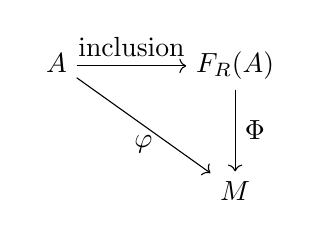
\begin{tikzpicture}
  \matrix (m)
    [
      matrix of math nodes,
      row sep    = 3em,
      column sep = 4em
    ]
    {
	    A & F_R(A) \\
	     & M            \\
    };
  \path
  (m-1-2) edge [->] node [right] {\(\Phi \)} (m-2-2)
    (m-1-1.east |- m-1-2)
    edge [->] node [above] {inclusion} (m-1-2)
      (m-1-1) edge [->] node [below] {$\varphi$} (m-2-2);
\end{tikzpicture}
\end{center}
Furthermore, if \(A = \left\{ a_1,\ldots,a_n \right\} \), then
\begin{align*}
	F_R(A) = Ra_1 \oplus Ra_2 \oplus \ldots \oplus Ra_n \stackrel{R}{\cong} R^{n}
\end{align*}
\end{thm}
This corresponds to the notion of free groups from group theory.

\begin{hw}
	If \(F_R,F_R'\) are free modules on the same set \(A\), there is a unique isomorphism between \(F_R\) and \(F_R'\) which is the identity map on \(A\).\\

	If \(\prescript{}{R}F\) is any free \(R\)-module with basis \(A\), then \(\prescript{}{R}F \cong F_R(A)\).
\end{hw}
If we have a free \(R\)-module with a basis \(A\), the above statement says that we can define \(R\)-module homomorphisms from the free module into other \(R\)-modules by simply specifying how the homomorphism acts on elements of \(A\).\\

The free module \(F_\Z(A)\) is called the \textbf{free abelian group on \(A\)}. If \(A\) is finite, then we say it is of \textbf{rank \(\left| A \right| \)} and is isomorphic to
\begin{align*}
	\Z \oplus \ldots^{n} \oplus \Z.
\end{align*}

%---
%
%diagonalizaton of modules etc
%
%---

\end{document}


\chapter{Group Representation Theory}
\label{cha:group_representation_theory}

\section{Ties to Group Representation Theory}
\label{sec:ties_to_group_representation_theory}
\documentclass{memoir}
\usepackage{notestemplate}

%\logo{~/School-Work/Auxiliary-Files/resources/png/logo.png}
%\institute{Rice University}
%\faculty{Faculty of Whatever Sciences}
%\department{Department of Mathematics}
%\title{Class Notes}
%\subtitle{Based on MATH xxx}
%\author{\textit{Author}\\Gabriel \textsc{Gress}}
%\supervisor{Linus \textsc{Torvalds}}
%\context{Well, I was bored...}
%\date{\today}

\begin{document}

% \maketitle

% Notes taken on 02/12/21


If, when taking an \(R\)-module \(M\), we may work over a field \(K\) and modify \(M = V\) to be a \(K\)-vector space by \(K\times V\to V\). This then gives us that an \(R\)-module over \(V\) is a pair \(V\) with \(R\times V\to V\).

\begin{defn}[Group Module]
	Let \(G\) be a group. We say that a \(K\)-vector space \(V\) is a \textbf{\(G\)-module} if it comes equipped with a \(G\)-action map
	\begin{align*}
		G\times V \to V \quad (g,v) \mapsto g*v :=gv
	\end{align*}
	compatible with operations of \(G\) and \(V\) :
	\begin{enumerate}[(a).]
		\item \(e_G v = v\) 
		\item \((gh)v = g(hv)\) 
		\item \(g(v+w) = gv + gw\) 
		\item \(g(\lambda v) = \lambda (gv)\)
	\end{enumerate}
	for all \(g,h \in G\), \(v \in V\), \(\lambda \in K\).
\end{defn}
If one is given a \(G\)-module \(V\), then there is a natural group homomorphism
\begin{align*}
	\rho:G\to \textrm{End}_K(V)\\
	g\mapsto \left[ \rho g : V \to V , \; v\mapsto g * v := gv \right] 
\end{align*}
The image of \(\rho\) is inside of \(GL(V)\).

\begin{defn}
	A \textbf{\(K\)-linear representation of a group \(G\)} is a \(K\)-vector space \(V\) equipped with a group homomorphism \(\rho:G \to GL(V)\).
\end{defn}

% Save recap

\begin{defn}
	Given a representation of a group \(G\), \((V:\rho)\), its \textbf{degree} is \(\textrm{dim}V\).
\end{defn}
Note that when \(\textrm{dim}_KV=n\), we get that
\begin{align*}
	GL(V) \cong GL_n(K)
\end{align*}
as groups.

% Something about V basis and maps between them?

Representations of \(G\) of degree \(n\) over a field \(K\) are congruent to group homomorphisms \(\rho:G\to GL_n(K)\).

\begin{defn}
	For any group \(G\), the \textbf{trivial representation of \(G\) over \(K\)} is \((V=K, \rho:G\to GL_1(K)=K^{\times })\) given by \(g\mapsto 1_K\) for all \(g \in G\).
\end{defn}

% Examples

\begin{defn}
	Let \(\rho:G\to GL(V)\) and \(\rho':G\to GL(V')\) be two representatives of a group \(G\). We say that \(p\) and \(p'\) are \textbf{equivalent} or isomorphic if there exists an invertible linear transformation
	\begin{align*}
		\tau:V\to V'
	\end{align*}
	so that \(\tau\) \textbf{intertwines} with action of \(G\) :
	\begin{align*}
		\tau(\rho g(v)) = \rho'g(\tau(v)) \quad \forall g \in G, v \in V
	\end{align*}
\end{defn}

\begin{rmrk}
	\(\rho:G\to GL_n(K)\) and \(\rho':G\to GL_{n'}(K)\) are equivalent if and only if \(n = n'\) and \(\exists T \in GL_n(K)\) such that \(T\rho(g)T^{-1} = \rho'(g)\) for all \(g \in G\).
\end{rmrk}
This notion will be captured more clearly later with homomorphism/isomorphisms.
\end{document}

\documentclass{memoir}
\usepackage{notestemplate}

%\logo{~/School-Work/Auxiliary-Files/resources/png/logo.png}
%\institute{Rice University}
%\faculty{Faculty of Whatever Sciences}
%\department{Department of Mathematics}
%\title{Class Notes}
%\subtitle{Based on MATH xxx}
%\author{\textit{Author}\\Gabriel \textsc{Gress}}
%\supervisor{Linus \textsc{Torvalds}}
%\context{Well, I was bored...}
%\date{\today}

\begin{document}

% \maketitle

% Notes taken on 02/22/21

\section{Subrepresentations and Irreducibility}
\label{sec:subrepresentations_and_irreducibility}

Let \(K\) be a field and \(G\) a group. Recall that if \(\textrm{dim}_KV = n\), we can identify the group \(GL(V)\) with \(GL_n(K)\), the group of invertible \(K \)-linear operators on \(V\) under composition.

\begin{defn}[Subrepresentations]
	Let \(\rho:G\to GL(V)\) be a representation of \(G\). Suppose that \(W\) is a subspace of \(V\) which is \(G\)-invariant. That is, for all \(w \in W\), \(g \in G\), it holds that  \(\rho_g(w)\in W\). Then \(W\) becomes a representation of \(G\) and we say that
	\begin{align*}
		(W,\rho w:G\to GL(W))\\
		g\mapsto \left[ \rho_g\mid W:W\to W \quad w \mapsto \rho_g(w) \right] 
	\end{align*}
	is a \textbf{subrepresentation} of \((V,\rho)\).
\end{defn}

% Examples

\begin{defn}
	The \textbf{direct sum} of two representations of \(G\), \((V',\rho_V')\) and \((V'',\rho_V'')\) is the representation of \(G\) given by:
	\begin{align*}
		(V:=V'\bigoplus V'', \rho_{V'\bigoplus V''}:G \to GL(V) )\\
		g\mapsto \left[ \rho_g:V\to V \quad v = v'+v''\mapsto \rho_g'(v') + \rho_g''(v'') \right] 
	\end{align*}
\end{defn}
If we fix a basis for both \(V'\) and \(V''\), then their union is a basis of \(V = V'\bigoplus V''\).

% Examples

\begin{defn}[Irreducible]
	A representation is called \textbf{irreducible} if it contains no proper subrepresentations-- otherwise it is called \textbf{reducible}. A representation is called \textbf{completely reducible} if it decomposes as a direct sum of irreducible subrepresentations.
\end{defn}
Irreducible representations will turn out to be the building blocks of group representation theory. This is complemented by Mascinke's Theorem, which will state that every \(\C\)-linear representation of a finite group \(G\) of finite degree is completely reducible.

% Example (Necessary)

\end{document}

\documentclass{memoir}
\usepackage{notestemplate}

%\logo{~/School-Work/Auxiliary-Files/resources/png/logo.png}
%\institute{Rice University}
%\faculty{Faculty of Whatever Sciences}
%\department{Department of Mathematics}
%\title{Class Notes}
%\subtitle{Based on MATH xxx}
%\author{\textit{Author}\\Gabriel \textsc{Gress}}
%\supervisor{Linus \textsc{Torvalds}}
%\context{Well, I was bored...}
%\date{\today}

\begin{document}

% \maketitle

% Notes taken on 02/24/21

\section{Complete Reducibility}
\label{sec:complete_reducibility}

Recall that the \textbf{characteristic} of a field \(K\) is the smallest positive integer \(p\) such that \(p 1_K = 0\). If \(p\) exists, then it is prime; else we say \(K\) has characteristic 0.

\begin{thm}
	Let \((V,\rho)\) be a representation of a finite group \(G\) of finite degree \(n\) over a field \(K\) of characteristic \(p\) with \(p \not\mid \left| G \right| \). If \(W\) is a subrepresentation of \((V,\rho)\), then there exists another subrepresentation \(W'\) of \(V\) so that
	\begin{align*}
		V \cong W \bigoplus W'
	\end{align*}
	as \(K\)-vector spaces. We refer to \(W'\) as the \textbf{complement} of the subrepresentation \(W\) of \((V,\rho)\).
\end{thm}

\begin{cor}[Maschke's Theorem]
	Let \(V\) be a representation of a finite group \(G\) of finite degree over a field of characteristic \(p\) with \(p \not\mid \left| G \right| \). Then \(V\) is completely reducible.
\end{cor}

This can be proven by induction on \(\textrm{dim}V\). Note that this fails for infinite groups.

\end{document}

\documentclass{memoir}
\usepackage{notestemplate}

%\logo{~/School-Work/Auxiliary-Files/resources/png/logo.png}
%\institute{Rice University}
%\faculty{Faculty of Whatever Sciences}
%\department{Department of Mathematics}
%\title{Class Notes}
%\subtitle{Based on MATH xxx}
%\author{\textit{Author}\\Gabriel \textsc{Gress}}
%\supervisor{Linus \textsc{Torvalds}}
%\context{Well, I was bored...}
%\date{\today}

\begin{document}

% \maketitle

% Notes taken on 02/26/21

\section{G-homomorphisms}
\label{sec:g_homomorphisms}

Let \(K\) be a field and \(G\) be a group. We are going to look at a structure of interest: we define \(K\)-linear representations of \(G\) as a \(K\)-vector space \(V\) equipped with a group homomorphism
\begin{align*}
	\rho:G\to GL(V)\\
	g\mapsto [\rho g:V\to V]
\end{align*}

\begin{defn}[\(G\)-homomorphism]
	Let \((V',\rho')\) and \((V'',\rho'')\) be representations of \(G\) over \(K\). A \textbf{\(G\)-homomorphism from \((V',\rho')\) to \(V'',\rho'')\)} is a \(K\) linear map \(\varphi:V'\to V''\) which intertwines with the action of \(G\) :
	\begin{align*}
		\varphi(\rho'g(v')) = \rho''g(\varphi(v')) \quad \forall g \in G, v' \in V'
	\end{align*}
	We denote the collection of \(G\)-homomorphisms from \((V', \rho')\) to \((V'', \rho'')\) by \( \textrm{Hom}_G(V',V'')\), and \(\textrm{End}_G(V') := \textrm{Hom}_G(V',V')\). Finally, a \textbf{\(G\)-isomorphism} is an invertible \(G\)-homomorphism.
\end{defn}

This is really just a change in basis.

\begin{prop}
	If \(\varphi \in \textrm{Hom}_G(V,W)\), then \(\varphi^{-1} \in \textrm{Hom}_G(W,V)\).
\end{prop}
\begin{prop} %Exercise 1 on HW 5
	Take \(\varphi \in \textrm{Hom}_G(V,W)\). Then
	\begin{enumerate}[(a).]
		\item \(\textrm{Ker}\varphi \) is a subrepresentation of \(V\), and
		\item \(\textrm{Im}\varphi\) is a subrepresentation of \(W\).
	\end{enumerate}
\end{prop}
For the rest of the section, we take \(K = \C\).

\begin{lemma}[Schur's Lemma]
	Let \((V,\rho)\) be an irreducible representation of \(G\). If \(\varphi \in \textrm{End}_G(V)\), then \(\varphi\) is a scalar multiple of \(\textrm{Id}V\) :
	\begin{align*}
		\exists \lambda \in \C \; s.t. \; \varphi(v) = \lambda v \quad \forall v \in V
	\end{align*}
\end{lemma}
This result has many applications.
\begin{thm}
	All nonzero complex irreducible representations of an abelian group \(G\) have degree 1.
\end{thm}
Using these tools, we now can complete a few problems.

\begin{hw}
	Given a finite abelian group \(G\), describe its irreducible representations, up to equivalence. Illustrate this for the Klein-four group \(G = C_2\times C_2\).
\end{hw}
Moreover, one can apply Schur's lemma to complete the following problem:
\begin{hw}
	Let \(V\) and \(W\) be irreducible representations of \(G\), and take \(\varphi \in \textrm{Hom}_G(V,W)\). Show that
	\begin{enumerate}[(a).]
		\item If \(V \not\cong W\), then \(\varphi\) is the zero map.
		\item If \(V \cong W\) and \(\varphi\neq 0\), then \(\varphi\) is a \(G\)-isomorphism.
	\end{enumerate}
\end{hw} % Hint: hw5 exercise 1

\end{document}

\documentclass{memoir}
\usepackage{notestemplate}

%\logo{~/School-Work/Auxiliary-Files/resources/png/logo.png}
%\institute{Rice University}
%\faculty{Faculty of Whatever Sciences}
%\department{Department of Mathematics}
%\title{Class Notes}
%\subtitle{Based on MATH xxx}
%\author{\textit{Author}\\Gabriel \textsc{Gress}}
%\supervisor{Linus \textsc{Torvalds}}
%\context{Well, I was bored...}
%\date{\today}

\begin{document}

% \maketitle

% Notes taken on ??


\section{Character Theory}
\label{sec:character_theory}

Character theory will serve as a very convenient bookkeeping tool for representations of \(G\) when \(G\) is finite. We still keep \(K = \C\).

\begin{defn}
	Let \((V,\rho)\) be a \(\C\)-representation of \(G\) of finite degree \(n\). Choose any basis of \(V\) and express \(\rho_g\) as a matrix in \(GL_n(\C)\), for all \(g \in G\). The \textbf{character of \((V,\rho)\)}, denoted \(X_V\) is the function
	\begin{align*}
		X_V:G\to \C\\
		g\mapsto \textrm{Tr}(\rho g)
	\end{align*}
	We say that \(X_V\) is \textbf{irreducible} if \((V,\rho)\) is irreducible.
\end{defn}
It turns out that characters detect irreducibility. Let \(X_V,\psi_W\) be given. We define a scalar by
\begin{align*}
	\langle X_V,\psi_W \rangle := \frac{1}{\left| G \right| }\sum_{g \in G} \overline{X_V(g)}\psi_W(g).
\end{align*}
\begin{prop}
	Let \(V\) be a representation of \(G\). Then
	\begin{align*}
		V \text{ is irreducible }\iff\langle X_V,X_V \rangle =1.
	\end{align*}
\end{prop}

Of course, we need to be sure that our construction of characters is well-defined. It turns out that they capture the properties of our representation well and are unique.

\begin{prop}
	\begin{enumerate}
		\item The definition of \(X_V\) is independent of choice of basis of \(V\)
		\item If \(V \cong W\), then \(X_V = X_W\) 
		\item If \(g,h \in G\) are conjugate, then \(X_V(g) = X_V(h)\)
	\end{enumerate}
\end{prop}

\begin{defn}
	The \textbf{character table} of \(G\) is defined as
	\begin{align*}
		\begin{bmatrix} X_{V_1}(g_1) & X_{V_1}(g_2) & \ldots & X_{V_1}(g_k)\\
		\vdots & & & \vdots \\
	X_{V_\ell}(g_1) & X_{V_\ell}(g_2) & \ldots & X_{V_\ell}(g_k)\end{bmatrix} 
	\end{align*}
\end{defn}
The number of irreducible characters of \(G\) is the same as the number of conjugacy classes of elements of \(G\). Furthermore, the character table is a square matrix with entries in \(\C\) when the rows are indexed by irreducible representations of \(G\) and the columns are indexed by conjugacy classes representations of elements of \(G\).\\

In this case, \((X_{V_i}(g_j))\) is an invertible matrix.

% Examples

\begin{prop}
	Let \((V,\rho )\) be a representation of \(G\), and take \(g \in G\). Then
	\begin{enumerate}
		\item \(X_V(e) = \textrm{dim}(V)\) 
		\item \(X_V(g)\) is a sum of roots of unity
		\item \(X_{V\oplus W}(g) = X_{V}(g) + X_{W}(g)\)
		\item \(X_V(g^{-1}) = \overline{X_V(g)}\) 
		\item \(\overline{X_V}\) is a character of \(G\)
	\end{enumerate}
\end{prop}

Let \(X_1,\ldots,X_r\) be irreducible characters of a finite group \(G\). Define
\begin{align*}
	\langle X_i, X_j \rangle := \frac{1}{\left| G \right| } \sum_{g \in G} \overline{X_i(g)}X_j(g)
\end{align*}

\begin{thm}
	\begin{enumerate}
		\item \(\langle X_i, X_j \rangle = \delta _{ij}\) 
		\item 
			\begin{align*}
				\sum_{i=1}^{r} \overline{X_i(x)}X_i(y) = \begin{cases}
					\left| C_G(x) \right| & x,y \text{ conjugate in }G\\
					0 & \text{otherwise}
				\end{cases}
			\end{align*}
	\end{enumerate}
\end{thm}
			Here, \(C_G(x)\) is the centralizer of \(x \in G\), that is, \(C_G(x) = \textrm{Stab}_x(G) = \left\{g \in G \mid g x g^{-1} = x \right\} \).

% Example

\begin{thm}
	If \(V,W\) are irreducible representations of \(G\), then
	\begin{align*}
		\langle X_V,X_V \rangle = 1\\
		\langle X_V,X_W \rangle = 0 \text{ when }V\not\cong W
	\end{align*}
\end{thm}
This shows us that characters completely determine representations, and forthermore characters completely determine irreducibility.
\end{document}


\chapter{Field Extensions}
\label{cha:field_extensions}

\documentclass{memoir}
\usepackage{notestemplate}

%\logo{~/School-Work/Auxiliary-Files/resources/png/logo.png}
%\institute{Rice University}
%\faculty{Faculty of Whatever Sciences}
%\department{Department of Mathematics}
%\title{Class Notes}
%\subtitle{Based on MATH xxx}
%\author{\textit{Author}\\Gabriel \textsc{Gress}}
%\supervisor{Linus \textsc{Torvalds}}
%\context{Well, I was bored...}
%\date{\today}

\begin{document}

% \maketitle

% Notes taken on ??

Recall the definition of a field.
\begin{defn}
	A \textbf{field} is a commutative ring \(F\) with multiplicative identity \(1_F\) in which every nonzero element has a multiplicative inverse.
\end{defn}
Furthermore, recall that the \textbf{characteristic} of a field \(F\), denoted \(\textrm{char}(F)\), is the smallest positive integer \(n\) such that
\begin{align*}
	1_F + 1_F + \ldots_n + 1_F = 0_F
\end{align*}
if such an \(n \in \N\) exists. Otherwise, we say that \(\textrm{char}(F)=0\).

\begin{prop}
	For a field \(F\), we have that \(\textrm{char}(F)=0\) or \(\textrm{char}(F) = p\) for a prime integer \(p\). If \(\textrm{char}(F) = p\), then \(p\cdot \alpha  = \alpha + \ldots_p + \alpha  = 0_F\) for all \(\alpha  \in F\).
\end{prop}
We often refer to fields with prime characteristics as \textbf{fields of positive characteristic}.\\

Some fields of characteristic zero include \(\Q\), \(\R\), and \(\C\). Any field of the form \(\Z / p\Z := \mathbb{F}_p\) is a field of characteristic \(p\).

\section{Subfields}
\label{sec:subfields}

\begin{defn}
	A \textbf{subfield} of a field \(F\) is a nonempty subset \(S\) containing \(1_F\) that is a subring under the addition and multiplication of \(F\), and so that \(S\) is closed under taking multiplicative inverse.\\

	The \textbf{prime subfield} of a field \(F\) is the subfield generated by the multiplicative identity \(1_F\) of \(F\), that is, it is the smallest subfield of \(F\) containing \(1_F\).
\end{defn}

\begin{prop}
	The prime subfield of a field \(F\) is either \(\Q\) if \(\textrm{char}(F) = 0\), or \(\mathbb{F}_p\) if \(\textrm{char}(F) = p\).
\end{prop}

\begin{defn}
	A \textbf{homomorphism \(\Phi:F_1\to F_2\) between fields \(F_1\) and \(F_2\)} is a unital ring homomorphism: \(\forall x,y \in F_1\)
	\begin{align*}
		\varphi (x+y) = \varphi (x) + \varphi (y)\\
		\varphi (xy) = \varphi (x) \varphi (y), \quad \varphi (1_{F_1}) = 1_{F_2}
	\end{align*}
\end{defn}
Notice that either \(F \cong \textrm{Im}(\varphi )\) or \(0 \cong \textrm{Im}(\varphi )\). This follows from the fact that the only ideals of \(F\) are \(0\) and \(F\).

A lot of fields are better viewed via a ring homomorphism. We can quotient out a ring \(R\) by any maximal ideal \(I\) of \(R\) to get an object isomorphic to a field.
\begin{exmp}
	Consider the principal ideal domain \(\Q[x]\). For any irreducible polynomial \(p(x)\), we have that
	\begin{align*}
		\Q[x] / (p(x))
	\end{align*}
	is a field, where \((p(x))\) denotes the root of \(p(x)\). We can in fact see that this space is equivalent to \(\Q\) but including the roots of \(x^2-2\), namely \(\sqrt{2} \). One can construct a unital isomorphism so that
	\begin{align*}
		\Q[x] / (x^2-2) \cong \Q(\sqrt{2} )
	\end{align*}
\end{exmp}

\end{document}

\documentclass{memoir}
\usepackage{notestemplate}

%\logo{~/School-Work/Auxiliary-Files/resources/png/logo.png}
%\institute{Rice University}
%\faculty{Faculty of Whatever Sciences}
%\department{Department of Mathematics}
%\title{Class Notes}
%\subtitle{Based on MATH xxx}
%\author{\textit{Author}\\Gabriel \textsc{Gress}}
%\supervisor{Linus \textsc{Torvalds}}
%\context{Well, I was bored...}
%\date{\today}

\begin{document}

% \maketitle

% Notes taken on 03/08/21

\section{Extension of Fields}
\label{sec:extension_of_fields}

\begin{defn}
	If \(K\) is a field containing a subfield \(F\), then \(K\) is said to be an \textbf{extension of \(F\)}, denoted by \(K / F\).\\

	The field \(F\) is sometimes called the \textbf{base field} of the extension.
\end{defn}
Note that if \(K\) is an extension of a field \(F\), then \(K\) is a \(F\)-vector space via the typical \(F\) action.

\begin{defn}
	The \textbf{degree} or \textbf{index} of a field extension \(K / F\), denoted \([K:F]\), is defined to be \(\textrm{dim}_F K\), the dimension of \(K\) as an \(F\)-vector space.
\end{defn}
For example, \([\Q(\sqrt{2} ) : \Q] = 2\) and \([\C: \R] = 2\). One can see the latter example by observing that \(\C\cong \R[x] / (x^2+1)\).

% Recall that we denote by \(F(\theta )\) the field \(F\) adjoined by the root \(\theta \), which is spanned by powers of \(\theta \) as an \(F\)-vector space.
\begin{thm}
	Let \(F\) be a field and \(p(x) \in F[x]\) be an irreducible polynomial. Then \(\exists \) a field extension \(K\) of \(F\) in which \(p(x)\) has a root.
\end{thm}
This field is given by \(K := F[x] / (p(x))\), but we will show this more formally later.

\begin{thm}
	Let \(p(x) \in F[x]\) be an irreducible polynomial of degree over \(F\), and let \(K\) be the field \(F[x] / (p(x))\). Take \(\theta := x + (p(x))\) (root of \(p(x)\) ). Then
	\begin{enumerate}
		\item The elements \(\left\{ 1_F, \theta , \theta ^2, \ldots, \theta ^{n-1} \right\} \) are an \(F\)-vector space basis of the \(F\)-vector space \(K\).
		\item \([K:F] = n\) 
		\item \(K = \left\{a_0 + a_1\theta + a_2\theta^2 + \ldots + a_{n-1}\theta ^{n-1} \mid a_0,\ldots,a_{n-1} \in F \right\} \) as an \(F\)-vector space.
	\end{enumerate}
\end{thm}
Another nice example to be familiar with is \(K = \mathbb{F}_2[x] / (x^2+x+1)\). This is a field extension of \(\mathbb{F}_2\) as \(x^2+x+1\) is irreducible in \(\mathbb{F}_2\). We can see that \([\mathbb{F}_2[x] / (x^2+x+1) : \mathbb{F}_2[x]] = 2\) simply because the degree of the polynomial is \(2\), but we can also directly count elements in the set and see that it has twice the elements of \(\mathbb{F}_2[x]\).\\

Now let's define fields formed by adjoining roots more formally.

\begin{defn}
	Let \(K / F\) be a field extension, and let \(\alpha_1,\alpha_2,\ldots \in K\) be elements. The smallest subfield of \(K\) containing both \(F\) and the elements \(\alpha_1,\alpha_2,\ldots,\) denoted \(F(\alpha_1,\alpha_2,\ldots)\) is called the \textbf{field generated by \(\alpha_1, \alpha_2,\ldots\) over \(F\)}.
\end{defn}

\begin{defn}
	The field \(F(\alpha )\) generated by a single element \(\alpha \) over \(F\) is called a \textbf{simple extension of \(F\)}, and the element \(\alpha \) in this case is called \textbf{primitive}.
\end{defn}

\begin{thm}
	Let \(F\) be a field and let \(p(x) \in F[x]\) be an irreducible polynomial. Suppose \(K\) is an extension of \(F\) containing a root \(\alpha \) of \(p(x)\). Then \(F[x] / (p(x)) \cong F(\alpha )\).
\end{thm}
It is natural to view field extensions as the base field appended with roots, and as a result a few definitions arise.

\begin{defn}[Algebraic and Transcendental Elements]
	An element \(\alpha \in K\) is called \textbf{algebraic over \(F\)} if \(\alpha \) is a root of some nonzero polynomial \(f(x) \in F[x]\).\\

	If \(\alpha  \in K\) is not algebraic over \(F\), then we say that \(\alpha \) is \textbf{transcendental over \(F\)}.
\end{defn}
The extension \(K / F\) is \textbf{algebraic over \(F\)} if all elements of \(K\) are algebraic over \(F\).

\begin{exmp}[Examples of Algebraic and Transcendental Elements]
	\begin{itemize}
		\item \(\sqrt{2} \) is an algebraic element over \(\Q\) via the polynomial \(x^2-2\). This actually holds for all \(\sqrt[n]{2} \) with \(x^{n}-2\).
		\item \(i\) is algebraic over \(\R\) and \(\Q\) via the polynomial \(x^2+1\) 
		\item Transcendental elements are much rarer-- examples include \(\pi \) and \(e\), but it is non-trivial to show an element is transcendental.
	\end{itemize}
\end{exmp}
\end{document}

\documentclass{memoir}
\usepackage{notestemplate}

%\logo{~/School-Work/Auxiliary-Files/resources/png/logo.png}
%\institute{Rice University}
%\faculty{Faculty of Whatever Sciences}
%\department{Department of Mathematics}
%\title{Class Notes}
%\subtitle{Based on MATH xxx}
%\author{\textit{Author}\\Gabriel \textsc{Gress}}
%\supervisor{Linus \textsc{Torvalds}}
%\context{Well, I was bored...}
%\date{\today}

\begin{document}

% \maketitle

% Notes taken on ??

\section{Minimal Polynomials}
\label{sec:minimal_polynomials}

\begin{prop}
	Let \(\alpha \) be an algebraic element over \(F\).
	\begin{enumerate}[(a).]
		\item Then there exists a monic irreducible polynomial of minimal degree \(m_{\alpha ,F}(x) \in F[x]\) which has \(\alpha \) as a root.
		\item A polynomial \(f(x) \in F[x]\) has \(\alpha \) as a root if and only if \(m_{\alpha ,F}(x) \mid f(x)\) in \(F[x]\).
		\item The polynomial \(m_{\alpha ,F}(x)\) with the property in (a) is unique.
	\end{enumerate}
\end{prop}
We can see the minimal polynomial must be irreducible, because otherwise one of its factors would have \(\alpha \) as a root and hence has degree smaller than \(m_{\alpha ,F}(x)\), contradicting our hypothesis. The divisibility \(m_{\alpha ,F}(x) \mid f(x)\) follows from the division algorithm in \(F[x]\). The divisibility and minimality conditions together give uniqueness.
\begin{cor}
	If \(K / F\) is a field extension, and \(\alpha \) is algebraic over both \(F\) and \(K\), then \(m_{\alpha ,K}(x)\) divides \(m_{\alpha ,F}(x)\) in \(K[x]\).
\end{cor}
This directly follows as \(m_{\alpha ,F}(x)\) has a root \(\alpha \) in \(K\) and hence (b) gives us divisibility.
\begin{defn}
	The polynomial \(m_{\alpha ,F}(x)\) is called the \textbf{minimal polynomial of \(\alpha \) over \(F\)}. The degree of \(m_\alpha (x)\) is called the \textbf{degree of \(\alpha \)}.\\

In other words, the minimal polynomial of \(\alpha \) over \(F\) is a monic irreducible polynomial over \(F\) that has \(\alpha \) as a root. Alternatively, it is a monic polynomial over \(F\) of minimal degree with \(\alpha \) as a root-- both imply the other.
\end{defn}

\begin{prop}
	Let \(\alpha \) be algebraic over \(F\). Then
	\begin{align*}
		F(\alpha ) \cong F[x] / (m_{\alpha }(x))
	\end{align*}
	So that \([F(\alpha ):F] = \textrm{deg}m_{\alpha }(x) \equiv \textrm{deg}\alpha\).
\end{prop}

\begin{prop}
	An element \(\alpha  \in F\) is algebraic over \(F\) if and only if the simple extension \(F(\alpha ) / F\) is finite.\\

	If \(\alpha \in K\) with \([K:F] = n\), then \(\textrm{deg}(\alpha) \leq n\).
\end{prop}
This follows by applying linear dependence to powers \(\alpha^i\) with \(i = 0,1,\ldots,n\).
\begin{cor}
	If \(K / F\) is finite, then \(K / F\) is algebraic.
\end{cor}

\begin{exmp}
	Take \(F\) to be a field with \(\textrm{char}(F) \neq 2\). Consider \(K/F\) of degree 2, which is hence algebraic. Let \(\alpha  \in K / F\) so that \(\alpha \) is a root of a polynomial over \(F\) of degree 1 or 2. Because \(\alpha \not\in F\), the polynomial must has degree 2.\\

	This implies that \(m_{\alpha ,F}(x) = x^2+bx+c\) for \(b,c \in F\). This implies that \(F(\alpha )\) has the same dimension of \(K\) and hence \(K = F(\alpha )\) (as \(K\) is a field extension of \(F(\alpha )\). This implies that \(K = F(\sqrt{b^2-4ac} )\) and so any degree 2 extension of a field \(F\) with characteristic not equal to \(2\) is of the form \(F(\sqrt{D} )\) for \(D\) a non-square element of \(F\).\\

	Conversely, for such a field, \([F(\sqrt{D} ) : F] = 2\) and hence extensions of the form \(F(\sqrt{D} ) / F\) are called \textbf{quadratic extensions of \(F\)}.
\end{exmp}
\end{document}

\documentclass{memoir}
\usepackage{notestemplate}

%\logo{~/School-Work/Auxiliary-Files/resources/png/logo.png}
%\institute{Rice University}
%\faculty{Faculty of Whatever Sciences}
%\department{Department of Mathematics}
%\title{Class Notes}
%\subtitle{Based on MATH xxx}
%\author{\textit{Author}\\Gabriel \textsc{Gress}}
%\supervisor{Linus \textsc{Torvalds}}
%\context{Well, I was bored...}
%\date{\today}

\begin{document}

% \maketitle

% Notes taken on whenever

\section{Algebraic Extensions}
\label{sec:algebraic_extensions}

\begin{thm}[Tower Theorem]
	Let \(F \hookrightarrow E \hookrightarrow K\) be a composition of field extensions. Then \([K:F] = [K:E] [E:F]\).
\end{thm}
One can show this via vector space arguments (look at the bases of the spaces).
\begin{cor}
	If \(K / F\) is a finite extension, and \(E\) is a subfield of \(K\) containing \(F\), then \([E:F] \mid [K:F] \).
\end{cor}

\begin{exmp}
	Let 
\begin{align*}
	K &= \Q(\sqrt[6]{2} )\\
	E &= \Q(\sqrt{2} )\\
	F &= \Q
\end{align*} It follow directly from previous work that \([\Q(\sqrt[6]{2}) : \Q] = 6\) and \([\Q(\sqrt{2} ):\Q] = 2\). As for \(K / E\), the minimal polynomial is \(x^3-\sqrt{2} \), which gives \([\Q(\sqrt[6]{2} ): \Q(\sqrt{2} )] = 3\), which corresponds to what the tower theorem gives us.
\end{exmp}

\begin{defn}
	An extension \(K / F\) is called \textbf{finitely generated} if there exist elements \(\alpha_1, \alpha_2,\ldots,\alpha_n\) such that
	\begin{align*}
		K = F(\alpha_1, \alpha_2, \ldots, \alpha_n) \quad \text{for }n<\infty
	\end{align*}
	Such an extension can be obtained recursively via simple extensions.
\end{defn}
	We have that \(F(\alpha ,\beta ) = (F(\alpha ))(\beta )\), hence the definition above is consistent.
\begin{exmp}
	\begin{itemize}
		\item \(\Q(\sqrt[6]{2} ,\sqrt{2} ) = \left( \Q(\sqrt[6]{2} ) \right) (\sqrt{2} ) = \Q(\sqrt[6]{2} )\) because \(\sqrt{2} = (\sqrt[6]{2} )^3\).
		\item One can check that \(\Q(\sqrt{2} ,\sqrt{3} )\) is a proper field extension for both \(\Q(\sqrt{2} )\) and \(\Q(\sqrt{3} )\).
	\end{itemize}
\end{exmp}
\begin{thm}
	\(K / F\) is finite if and only if \(K\) is generated by a finite number of algebraic elements over \(F\).
\end{thm}
We denote by \(\overline{\Q}\) the subfield of \(\C\) generated by all algebraic elements of \(\C\) over \(\Q\). \(\overline{\Q}\) is an infinite algebraic extension of \(\Q\), and referred to as the \textbf{field of algebraic numbers}. \\

\begin{thm}
	If \(E / F\) and \(K / E\) are algebraic, then \(K / F\) is algebraic.
\end{thm}
\end{document}

\documentclass{memoir}
\usepackage{notestemplate}

%\logo{~/School-Work/Auxiliary-Files/resources/png/logo.png}
%\institute{Rice University}
%\faculty{Faculty of Whatever Sciences}
%\department{Department of Mathematics}
%\title{Class Notes}
%\subtitle{Based on MATH xxx}
%\author{\textit{Author}\\Gabriel \textsc{Gress}}
%\supervisor{Linus \textsc{Torvalds}}
%\context{Well, I was bored...}
%\date{\today}

\begin{document}

% \maketitle

% Notes taken on whenever

\section{Composite Field Extensions}
\label{sec:composite_field_extensions}

\begin{defn}[Composite Field]
	Let \(K_1\) and \(K_2\) be two subfields of a field \(K\). Then the \textbf{composite field of \(K_1\) and \(K_2\)}, denoted by \(K_1K_2\) is the smallest subfield of \(K\) containing both \(K_1\) and \(K_2\).
\end{defn}
The composite of any collection of subfields \(\left\{ K_i \right\} \) is defined similarly.\\\

\begin{prop}
	Let \(K_1\) and \(K_2\) be two finite extensions of \(F\) contained in \(K\). Then
	\begin{align*}
		[K_1K_2:F] \leq [K_1:F][K_2:F]
	\end{align*}
	with equality if and only if an \(F\)-vector space basis for \(K_1\) is linearly independent over \(K_2\) (or vice versa).
\end{prop}
If the \(F\)-vector space basis of \(K_1\) is \(\alpha_1,\ldots,\alpha_n\) and the \(F\)-vector space basis of \(K_2\) is \(\beta_1,\ldots,\beta_m\), then \(\left\{ \alpha_i \beta_j \right\}_{i,j = 1}^{n,m}\) is a \(F\)-vector span of \(K_1K_2\).
\begin{cor}
	If, furthermore, \([K_1:F] = n\) and \([K_2:F] = m\) with \(\textrm{gcd}(n,m) = 1\), then \([K_1K_2:F] = [K_1:F][K_2:F] = nm\).
\end{cor}

\begin{exmp}
	\begin{itemize}
		\item Consider \(K = \Q(\sqrt{2} )\Q(\sqrt[3]{2}) \). We have
			\begin{align*}
				\Q &\hookrightarrow^{2} \Q(\sqrt{2} ) \hookrightarrow^{3} \Q(\sqrt{2})\Q(\sqrt[3]{2}) = \Q(\sqrt[6]{2})\\
				\Q &\hookrightarrow^{3} \Q(\sqrt[3]{2}) \hookrightarrow^{2} \Q(\sqrt[6]{2})\\
				\Q &\hookrightarrow^{6} \Q(\sqrt[6]{2})
			\end{align*}
			where \(\hookrightarrow^{k}\) represents a degree \(k\) extension. % Fill in rest of field extensions here, and perhaps turn into diagrams
	\end{itemize}
\end{exmp}

\section{Splitting Fields}
\label{sec:splitting_fields}

Recall that for any field \(F\) and any polynomial \(f(x) \in F[x]\), there exists a field extension \(K\) over \(F\) that contains a root, say \(\alpha  \in K\), of \(f(x)\). In this case, \(f(x) = (x-\alpha )g(x)\) in \(K[x]\) as \(K[x]\) is a Euclidean domain.\\

Now we want a field extension \(K / F\) so that \(f(x) \in F[x]\) splits completely into linear factors in \(K[x]\).

\begin{defn}
	A field extension \(K\) of \(F\) is called a \textbf{splitting field for \(f(x) \in F[x]\)} if \(f(x) = \prod_{i} (x - \alpha_i) \) in \(K[x]\) and \(f(x)\) does NOT factor completely in \(K'[x]\) for any proper subfield \(K'\) of \(K\).
\end{defn}
\(f(x) \in K[x]\) splits completely if and only if \(K\) contains all roots of \(f(x)\).

\begin{exmp}
	\begin{itemize}
		\item The splitting field of \(x^2-2\) over \(\Q\) is \(\Q(\sqrt{2} )\) 
		\item The splitting field of \((x^2-2)(x^2-3)\) over \(\Q\) is \(\Q(\sqrt{2} ,\sqrt{3} )\)
		\item The splitting field of \(x^3-2\) over \(\Q\) is NOT \(\Q(\sqrt[3]{2})\). The roots \(\sqrt[3]{2}\omega \) and \(\sqrt[3]{2}\omega^2 \) are in fact imaginary and hence are not in \(\Q(\sqrt[3]{2})\) (note that \(\omega \) represents the principal root of unity).
	\end{itemize}
\end{exmp}

\begin{thm}
	Splitting fields always exist. For any field \(F\), if \(f(x) \in F[x]\), then there exists a field extension \(K\) of \(F\) that is a splitting field for \(f(x)\).
\end{thm}
\end{document}

\documentclass{memoir}
\usepackage{notestemplate}

%\logo{~/School-Work/Auxiliary-Files/resources/png/logo.png}
%\institute{Rice University}
%\faculty{Faculty of Whatever Sciences}
%\department{Department of Mathematics}
%\title{Class Notes}
%\subtitle{Based on MATH xxx}
%\author{\textit{Author}\\Gabriel \textsc{Gress}}
%\supervisor{Linus \textsc{Torvalds}}
%\context{Well, I was bored...}
%\date{\today}

\begin{document}

% \maketitle

% Notes taken on 03/17/21

\begin{prop}
	Take \(f(x) \in F[x]\) of degree \(n\). Then for \(K :=\) splitting field of \(f(x)\), we get that \([K:F] \leq n!\).
\end{prop}
Now we discuss the uniqueness of splitting fields.
\begin{thm}
	Let \(\varphi :F\to F'\) be an isomorphism of fields. Let
	\begin{align*}
		f(x) = a_nx^{n}+ \ldots + a_1x + a_0 \in F[x]\\
		f'(x) = \varphi (a_n)x^{n}+ \ldots + \varphi (a_1) x + \varphi (a_0) \in F'[x].
	\end{align*}
	Let \(E\) be the splitting field of \(f(x)\) over \(F\) and \(E'\) be the splitting field of \(f'(x)\) over \(F'\). Then the isomorphism \(\varphi \) extens to an isomorphism \(\sigma :E\to E'\), so that \(\sigma \mid_F = \varphi \).
\end{thm}
This can be proven by induction on the degree of \(f(x)\).
\begin{cor}
	Any two splitting fields for a polynomial \(f(x) \in F[x]\) over a field \(F\) are isomorphic.
\end{cor}

Thus we can safely refer to -the- splitting field of a polynomial over a field.

\begin{defn}
	If \(K\) is an algebraic extension of \(F\), which is the splitting field over \(F\) for a collection of polynomials \(\left\{ f_i(x) \right\} \in F[x]\), then \(K\) is called a \textbf{normal} extension of \(F\).
\end{defn}
In other words, a normal extension is simply an algebraic extension that is also a splitting field.
\begin{hw}
	Determine the splitting field of \(x^{6}-4\) over \(\Q\) and its degree over \(\Q\).
\end{hw}
\end{document}

\documentclass{memoir}
\usepackage{notestemplate}

%\logo{~/School-Work/Auxiliary-Files/resources/png/logo.png}
%\institute{Rice University}
%\faculty{Faculty of Whatever Sciences}
%\department{Department of Mathematics}
%\title{Class Notes}
%\subtitle{Based on MATH xxx}
%\author{\textit{Author}\\Gabriel \textsc{Gress}}
%\supervisor{Linus \textsc{Torvalds}}
%\context{Well, I was bored...}
%\date{\today}

\begin{document}

% \maketitle

% Notes taken on 03/22/21

We now focus on the splitting field of \(x^{n}-1\) in \(\Q[x]\). Roots of \(x^{n}-1\) are of the form \(\left\{e^{2\pi i k / n} \mid k = 0,1,\ldots,n-1 \right\} \). Some useful notation:
\begin{enumerate}
	\item \(\zeta _n := e^{2\pi i / n}\), the primitive \(n\)-th root of 1
	\item \(\mu_n := \langle \zeta _n \rangle \), the cyclic group of order \(n\) under multiplication with identity 1
	\item \(\varphi (n)\) is the number of integers between \(1,\ldots,n\) that are coprime-- the Euler-Phi function.
\end{enumerate}

\begin{defn}[Cyclotomic Field]
	The \textbf{cyclotomic field of \(n\)-th roots of unity} or the \textbf{\(n\)-th cyclotomic field} is \(\Q(\zeta_n)\).\\

	The \textbf{\(n\)-th cyclometric polynomial} is
	\begin{align*}
		\Phi_n(x) = \prod_{\zeta \text{primitive} \in \mu_n} (x-\zeta ). 
	\end{align*}
\end{defn}
Recall that an \(n\)-th root of \(1\) (that is, \(e^{2\pi ik / n}\)) is primitive if and only if \((k,n) = 1\). We conventionally choose \(1\) to be a primitive.

\begin{thm}
	\begin{enumerate}[(a).]
		\item \(\Phi_n(x)\) is a monic polynomial in \(\Z[x]\) of degree \(\varphi (n)\) 
		\item \(\Phi_n(x) \in \Z[x]\) is irreducible
		\item The minimal polynomial of a primitive \(n\)-th root of unity over \(\Q\) is \(\Phi_n(x)\) 
		\item \([\Q(\zeta_n):\Q] = \varphi(n)\)
	\end{enumerate}
\end{thm}

These will be proved in various ways by later constructions.

\begin{cor}
	\begin{align*}
		\Phi_n(x) = (x^{n}-1) \big/ \prod_{d|n, d<n} \Phi_d(x) 
	\end{align*}
	We can compute \(\Phi_n(x)\) inductively.
\end{cor}
As an example, for a prime \(p\):
\begin{align*}
	\Phi_p(x) = \frac{x^{p}-1}{x-1} = x^{p-1}+ x^{p-2} + \ldots + x^2 + x + 1
\end{align*}
\end{document}

\documentclass{memoir}
\usepackage{notestemplate}

%\logo{~/School-Work/Auxiliary-Files/resources/png/logo.png}
%\institute{Rice University}
%\faculty{Faculty of Whatever Sciences}
%\department{Department of Mathematics}
%\title{Class Notes}
%\subtitle{Based on MATH xxx}
%\author{\textit{Author}\\Gabriel \textsc{Gress}}
%\supervisor{Linus \textsc{Torvalds}}
%\context{Well, I was bored...}
%\date{\today}

\begin{document}

% \maketitle

% Notes taken on 03/24/21

\section{Algebraic Closure}
\label{sec:algebraic_closure}

Before, we were looking at extensions of some polynomial in \(F[x]\) that contains all the roots of the polynomial. Now we consider field extensions that contain \textit{all} the roots of all \(f(x) \in F[x]\).

\begin{defn}[Algebraic Closure]
	Given a field \(F\), a field \(\overline{F}\) is the \textbf{algebraic closure} of \(F\) if
	\begin{enumerate}[(a).]
		\item \(\overline{F}\) is algebraic over \(F\),
		\item Every polynomial \(f(x) \in F[x]\) splits completely over \(\overline{F}\)
	\end{enumerate}
\end{defn}
Recall that splitting completely implies that \(f(x)\) factors into a product of degree 1 polynomials.

\begin{defn}[Algebraically Closed]
	A field \(K\) is \textbf{algebraically closed} if every polynomial with coefficients in \(K\) has a root in \(K\).
\end{defn}

\begin{prop}
	If \(\overline{F}\) is the algebraic closure of \(F\), then \(\overline{F}\) is algebraically closed.
\end{prop}

\begin{hw}
	For a field \(K\), the following are equivalent:
	\begin{itemize}
		\item \(K\) is algebraically closed
		\item Every \(f(x)\in K[x]\) nonconstant splits completely over \(K\) 
		\item Every irreducible \(f(x) \in K[x]\) has degree 1
		\item There does not exist an algebraic extension of \(K\) other than \(K\) itself
	\end{itemize}
\end{hw}

\begin{prop}
	For every field \(F\) there exists an algebraically closed field \(K\) containing \(F\).
\end{prop}

\begin{hw}% Dummitt-Foote 13.4 #5
	Let \(K\) be a finite extension of \(F\). Prove that \(K\) is a splitting field over \(F\) if and only if every irreducible polynomial in \(F[x]\) that has a root in \(K\) splits completely in \(K[x]\).
\end{hw}
\end{document}

\documentclass{memoir}
\usepackage{notestemplate}

%\logo{~/School-Work/Auxiliary-Files/resources/png/logo.png}
%\institute{Rice University}
%\faculty{Faculty of Whatever Sciences}
%\department{Department of Mathematics}
%\title{Class Notes}
%\subtitle{Based on MATH xxx}
%\author{\textit{Author}\\Gabriel \textsc{Gress}}
%\supervisor{Linus \textsc{Torvalds}}
%\context{Well, I was bored...}
%\date{\today}

\begin{document}

% \maketitle

% Notes taken on 03/29/21

\section{Separability}
\label{sec:separability}

\begin{defn}[Multiplicity]
	Take \(f(x) \in F[x]\). Then over a splitting field over \(F\), we get \(f(x) = (x-\alpha_1)^{n_1}(x-\alpha_2)^{n_2}\ldots(x-\alpha_k)^{n_k}\) where \(\alpha_1,\ldots,\alpha_k\) are distinct elements of the splitting field and \(n_1\geq 1\) for all \(i\). The value \(n_i\) is called the \textbf{multiplicity} of \(\alpha_i\), and if  \(n_i>1\), \(\alpha_i\) is a \textbf{multiple root} of \(f(x)\). If \(n_i=1\) instead, then we say that \(\alpha_i\) is a \textbf{simple root}.
\end{defn}

\begin{defn}[Separable polynomials]
	A polynomial \(f(x) \in F[x]\) is called \textbf{separable} if it has no multiple roots over a splitting field for \(F\). Else, \(f(x)\) is called \textbf{inseparable}.
\end{defn}

\begin{defn}[Polynomial derivative]
	If \(f(x) = a_n x^{n} + a_{n-1}x^{n-1} + \ldots + a_2 x^{2} + a_1x + a_0 \in F[x]\), then its \textbf{derivative} is
	\begin{align*}
		D_xf(x) = na_n x^{n-1}+ \ldots + 2a_2 x + a_1 \in F[x]
	\end{align*}
\end{defn}

\begin{prop}
	Take \(f(x) \in F[x]\) with root \(\alpha \). Then the multiplicity of \(\alpha \) is greater than one if and only if \(D_xf(\alpha ) = 0\).
\end{prop}
In other words, \(f(x)\) is separable when \(f(x)\) and \(D_xf(x)\) share no roots.

\begin{cor}
	\begin{enumerate}[(a).]
		\item Every irreducible polynomial over a field \(F\) of characteristic zero is separable
		\item A polynomial over a field of characteristic zero is separable if and only if it is the product of distinct irreducible factors
	\end{enumerate}
\end{cor}


Now we discuss how separability relates to field extensions.
\begin{defn}[Separable]
	Let \(K / F\) be a field extension. An element \(\alpha  \in K\) is \textbf{separable over \(F\)} if \(\alpha \) is algebraic over \(F\) and \(m_{\alpha ,F}(x)\) is separable.\\

	The extension \(K / F\) is \textbf{separable} if every element of \(K\) is separable over \(F\). If there is an \(\alpha  \in K\) that is not separable over \(F\), then \(K / F\) is an \textbf{inseparable} extension.
\end{defn}

\begin{prop}
	Every finitely generated algebraic extension of \(\Q\) is separable.
\end{prop}
\end{document}

\documentclass{memoir}
\usepackage{notestemplate}

%\logo{~/School-Work/Auxiliary-Files/resources/png/logo.png}
%\institute{Rice University}
%\faculty{Faculty of Whatever Sciences}
%\department{Department of Mathematics}
%\title{Class Notes}
%\subtitle{Based on MATH xxx}
%\author{\textit{Author}\\Gabriel \textsc{Gress}}
%\supervisor{Linus \textsc{Torvalds}}
%\context{Well, I was bored...}
%\date{\today}

\begin{document}

% \maketitle

% Notes taken on 05-10-21

\section{Techniques in Characteristic p > 0}
\label{sec:techniques_in_characteristic_p_0}

\begin{prop}
	Let \(F\) be a field of characteristic \(p>0\). Then for all \(a,b \in F\), we get that
	\begin{align*}
		(a+b)^{p} = a^{p} + b^{p}\\
		(ab)^{p} = a^{p}b^{p}
	\end{align*}
\end{prop}
This is the "Freshman's Dream".

\begin{defn}[Frobenius Endomorphism]
	For a field \(F\) of characteristic \(p>0\), the function
	\begin{align*}
		\varphi :F\to F\\
		a\mapsto a^{p}
	\end{align*}
	is the \textbf{Frobenius endomorphism} of \(F\).
\end{defn}
\begin{cor}
	The Frobenius endomorphism of \(F\) is an injective field homomorphism. When \(F\) is finite, it is also surjective.
\end{cor}

Now we will go back to some propositions about finite fields using these ideas.
\begin{prop}
	Every irreducible polynomial over a finite field \(F\) is separable. Moreover, \(f(x) \in F[x]\) is separable if and only if it is the product of distinct irreducible polynomials in \(F[x]\).
\end{prop}
This follows by contradiction. One can express the irreducible polynomial as a polynomial of the form \(g(x^{p})\), but this polynomial can be shown to be reducible, and so cannot occur.

\begin{defn}[Perfect]
	A field \(K\) of characteristic \(p>0\) is called \textbf{perfect} if every element of \(K\) is a \(p\)-th power in \(K\)-- that is, \(K = K^{p}\).
\end{defn}
By convention any field of characteristic zero is also called perfect.\\

We have just shown that every irreducible polynomial over a perfect field is separable, and hence finite extensions of perfect fields are separable.

\begin{hw}
	Prove that there exists a non-perfect infinite field \(F\), i.e. find \(f(x) \in F[x]\) so that \(f\) is irreducible and not separable.
\end{hw}

These concepts can be used to prove that the \(n\)-th cyclotomic polynomial \(\Phi_n(x) \in \Z[x]\) is irreducible.

\end{document}

\documentclass{memoir}
\usepackage{notestemplate}

%\logo{~/School-Work/Auxiliary-Files/resources/png/logo.png}
%\institute{Rice University}
%\faculty{Faculty of Whatever Sciences}
%\department{Department of Mathematics}
%\title{Class Notes}
%\subtitle{Based on MATH xxx}
%\author{\textit{Author}\\Gabriel \textsc{Gress}}
%\supervisor{Linus \textsc{Torvalds}}
%\context{Well, I was bored...}
%\date{\today}

\begin{document}

% \maketitle

% Notes taken on 05/10/21

\begin{thm}
	Let \(K / \mathbb{F}_p\) be a field extension of the prime subfield \(\mathbb{F}_p\).
	\begin{itemize}
		\item If \(K\) is finite, then \(\left| K \right| = p^{n}\) for some positive integer \(n\).
		\item \(\left| K \right| = p^{n}\) if and only if \(K\) is the splitting field of \(x^{p^{n}}-x\) over \(\mathbb{F}_p\).
	\end{itemize}
	By the uniqueness of splitting fields, we can simply denote \(K\) by \(\mathbb{F}_{p^{n}}\).
\end{thm}
This theorem gives us a complete characterization of finite fields. The first part is proven in Dummitt-Foote 13.2 \#1.

\begin{cor}
	For all prime \(p\), for all \(n \in \Z_+\), there exists a field of cardinality \(p^{n}\). Furthermore, any two finite fields of the same cardinality are isomorphic.
\end{cor}

\section{Simple Extensions}
\label{sec:simple_extensions}

\begin{thm}
	If \(\left| F \right| < \infty\), and \(K / F\) is a finite extension of \(F\), then \(K = F(\alpha )\) for some \(\alpha  \in K\).	
\end{thm}

This holds because \(K^{\times }\) is a cyclic group, and so there must exist \(\alpha \) so \(\langle \alpha  \rangle = K^{\times }\), and hence \(K = F(\alpha )\).

\begin{thm}
	If \(F\) is an infinite field, and \(K / F\) is a finite separable extension, then \(K = F(\alpha )\) for some \(\alpha  \in K\).
\end{thm}
Every field extension can be written by appending a sequence of elements, and we can reduce the elements to one by the combination \(\alpha  = \beta + \gamma  \delta \), where \((\beta ,\gamma )\) is the two additional elements, and \(\delta \neq \frac{\beta_i - \beta }{\gamma  - \gamma_j}\). Often we can simply choose \(\delta =1\) if we are lucky.

\end{document}

\documentclass{memoir}
\usepackage{notestemplate}

%\logo{~/School-Work/Auxiliary-Files/resources/png/logo.png}
%\institute{Rice University}
%\faculty{Faculty of Whatever Sciences}
%\department{Department of Mathematics}
%\title{Class Notes}
%\subtitle{Based on MATH xxx}
%\author{\textit{Author}\\Gabriel \textsc{Gress}}
%\supervisor{Linus \textsc{Torvalds}}
%\context{Well, I was bored...}
%\date{\today}

\begin{document}

% \maketitle

% Notes taken on 05/10/21

\chapter{Galois Theory}
\label{cha:galois_theory}

Galois theory studies the connection between finite field extensions via roots of polynomials and the structures of groups that permute those roots.\\

Let \(F,K\) be fields, and \(K / F\) a field extension.

\begin{defn}[Field Automorphism]
	We say that \(\sigma :K\to K\) is a \textbf{field automorphism} if \(\sigma \) is a bijective unital ring homomorphism. We denote the collection of field automorphisms of \(K\) by \(\textrm{Aut}(K)\).\\

	An automorphism \(\sigma  \in \textrm{Aut}(K)\) \textbf{fixes an element} \(\alpha  \in K\) if \(\sigma (\alpha )=\alpha \).\\

	An automorphism \(\sigma \in \textrm{Aut}(K)\) \textbf{fixes a subset \(E\) of \(K\)} if \(\sigma (\alpha ) = \alpha \) for all \(\alpha  \in E\).\\

	For \(\sigma  \in \textrm{Aut}(K)\) and \(E\subset K\), \(\sigma (E)\) denotes the subset \(\left\{\sigma (\alpha ) \mid \alpha \in E \right\} \)
\end{defn}
Recall that the prime subfield of a field \(K\) is given by
\begin{align*}
	K_{\textrm{prime}} = \begin{cases}
		\Q & K \text{ has characteristic 0}\\
		\Z_p & \text{\(p\) prime}
	\end{cases}
\end{align*}
because \(\sigma \in \textrm{Aut}(K)\) fixes \(1_K\), it must hold that \(\sigma \) fixes \(K_{\textrm{prime}}\) and hence prime subfields are fixed by any automorphism of a field.

\section{Automorphisms fixing subfields}
\label{sec:automorphisms_fixing_subfields}

\begin{defn}
	We define \(\textrm{Aut}(K / F)\) to be the collection of automorphisms of \(K\) that fix \(F\).
\end{defn}

\begin{prop}
	\(\textrm{Aut}(K)\) is a group under composition, and \(\textrm{Aut}(K / F)\) is a subgroup of \(\textrm{Aut}(K)\).
\end{prop}

\begin{prop}
	Let \(\alpha  \in K\) be an algebraic element over \(F\). Then for any \(\alpha \in \textrm{Aut}(K / F)\), we get that \(m_{\alpha ,F}(\sigma (\alpha )) = 0\).
\end{prop}
In other words, automorphisms permute roots of minimal polynomials.

\section{Subfields and Subgroups}
\label{sec:subfields_and_subgroups}

\begin{prop}
	Let \(H\) be a subgroup of \(\textrm{Aut}(K)\). Then 
	\begin{align*}
		\left\{\alpha  \in K \mid \sigma (\alpha ) = \alpha \quad \forall \sigma \in H \right\} 
	\end{align*}
	is a subfield of \(K\). We call this subfield the \textbf{fixed field of \(H\)} denoted by \(K^{H}\).
\end{prop}

In fact, this structure induces a correspondence between field extensions and chains of subgroups.
\begin{prop}
	Let \(F_1 \subset F_2 \subset K\) be a sequence of field extensions. Then \(\textrm{Aut}(K / K) = \textrm{Id}_{\textrm{Aut}(K)} \leq \textrm{Aut}(K / F_2) \leq \textrm{Aut}(K / F_1)\).\\

	Conversely, let \(H_1 \leq H_2 \leq \textrm{Aut}(K)\) be a chain of subgroups. Then \(K^{\textrm{Aut}(K)} = K_{\textrm{prime}} \subset K^{H_2} \subset K^{H_1}\)
\end{prop}
\end{document}

\documentclass{memoir}
\usepackage{notestemplate}

%\logo{~/School-Work/Auxiliary-Files/resources/png/logo.png}
%\institute{Rice University}
%\faculty{Faculty of Whatever Sciences}
%\department{Department of Mathematics}
%\title{Class Notes}
%\subtitle{Based on MATH xxx}
%\author{\textit{Author}\\Gabriel \textsc{Gress}}
%\supervisor{Linus \textsc{Torvalds}}
%\context{Well, I was bored...}
%\date{\today}

\begin{document}

% \maketitle

% Notes taken on 05/10/21

\begin{prop}
	Let \(E\) be the splitting field over \(F\) of a polynomial \(f(x) \in F[x]\). Then
	\begin{align*}
		\left| \textrm{Aut}(E / F)\right|  \leq [E:F] 
	\end{align*}
	with equality if and only if \(f(x)\) is separable over \(F\).
\end{prop}
The techniques used to prove this proposition also tell us that if \(K / F\) is finite, then \(\left| \textrm{Aut}(K / F) \right| \leq [K:F]\).

\begin{defn}
	Let \(K / F\) be a finite extension.
	\begin{itemize}
		\item If \(\left| \textrm{Aut}(K / F) \right| = [K:F]\) then \(K\) is \textbf{Galois over \(F\)} and \(K / F\) is a \textbf{Galois extension}.
		\item If \(K / F\) is Galois, then the group \(\textrm{Aut}(K / F)\) is called the \textbf{Galois group} of \(K / F\) and is denoted \(\textrm{Gal}(K / F)\).
	\end{itemize}
\end{defn}
\end{document}

\documentclass{memoir}
\usepackage{notestemplate}

%\logo{~/School-Work/Auxiliary-Files/resources/png/logo.png}
%\institute{Rice University}
%\faculty{Faculty of Whatever Sciences}
%\department{Department of Mathematics}
%\title{Class Notes}
%\subtitle{Based on MATH xxx}
%\author{\textit{Author}\\Gabriel \textsc{Gress}}
%\supervisor{Linus \textsc{Torvalds}}
%\context{Well, I was bored...}
%\date{\today}

\begin{document}

% \maketitle

% Notes taken on 05/10/21

\begin{exmp}
	Let \(K = \Q(\sqrt{2} ,\sqrt{3} )\). Then one can see that \(\Q(\sqrt{2} )\), \(\Q(\sqrt{3} )\), and \(\Q(\sqrt{6} )\) are all subfields for which \(K\) is a Galois extension. Furthermore, these fields are all Galois extensions of \(\Q\).
\end{exmp}

\begin{exmp}
	Consider the quotient field \(\mathbb{F}_2(t)\) of \(\mathbb{F}_2[t]\) and consider \(f(x) = x^2-t \in \mathbb{F}_2(t)[x]\). One can show that \(f(x)\) is irreducible but not separable over \(\mathbb{F}_2(t)\), and hence if \(\theta \) is a root of \(f(x)\), \(\mathbb{F}_2(t)(\theta )\) is NOT a Galois extension of \(\mathbb{F}_2(t)\).
\end{exmp}

\begin{exmp}
	Let \(K\) be the splitting field of \(x^3-2\), i.e. \(K = \Q(\sqrt[3]{2} ,\omega )\). \(K\) is Galois over \(\Q\), but \(\Q(\sqrt[3]{2} )\) is NOT Galois over \(\Q\).\\

	In fact, \(\textrm{Gal}(K / \Q) \) is a nonabelian group of order 6, and thus is isomorphic to \(S_3\).
\end{exmp}
\end{document}

\documentclass{memoir}
\usepackage{notestemplate}

%\logo{~/School-Work/Auxiliary-Files/resources/png/logo.png}
%\institute{Rice University}
%\faculty{Faculty of Whatever Sciences}
%\department{Department of Mathematics}
%\title{Class Notes}
%\subtitle{Based on MATH xxx}
%\author{\textit{Author}\\Gabriel \textsc{Gress}}
%\supervisor{Linus \textsc{Torvalds}}
%\context{Well, I was bored...}
%\date{\today}

\begin{document}

% \maketitle

% Notes taken on 05/10/21

We can summarize our characterization thus far by a set of equivalences. The following are equivalent:
\begin{itemize}
	\item A finite field extension \(K / F\) is Galois
	\item \(\left| \textrm{Aut}(K / F) \right| = [K:F]\) 
	\item \(K / F\) is the splitting field of a separable polynomial over \(F\) 
	\item \(K / F\) is normal and separable
	\item \(F = K^{\textrm{Aut}(K / F)}\)
\end{itemize}

\section{Fundamental Theorem of Galois Theory}
\label{sec:fundamental_theorem_of_galois_theory}

\begin{thm}[Fundamental Theorem of Galois Theory]
	Let \(K / F\) be Galois and set \(G:= \textrm{Gal}(K / F)\). Then there exists a bijection between the subfields \(E\subset K\) with \(F\subset E\) and the subgroups \(H \leq G\) given by
\begin{align*}
	E \mapsto \textrm{Aut}(K / E)\\
	H \mapsto K^{H}
\end{align*}
and these maps are inverses of each other. Furthermore, this bijection has some additonal properties:
\begin{itemize}
	\item If \(E_1 \leftrightarrow H_1\) and \(E_2 \leftrightarrow H_2\), then \(E_1 \subset E_2 \iff H_2 \leq H_1\).
	\item If \(E \leftrightarrow H\), then \([K:E] = \left| H \right| \) and \([E:F] = [G:H]\).
	\item \(K / E\) is always Galois for \(F \subset E \subset  K\).
	\item \(E / F\) is Galois if and only if \(H \triangleleft G\). In this case, \(\textrm{Gal}(E / F) \cong G / H\).
	\item If \(E_1 \leftrightarrow H_1\) and \(E_2 \leftrightarrow H_2\), then \(E_1 \cap E_2 \leftrightarrow \langle H_1,H_2 \rangle \) and \(E_1E_2 \leftrightarrow H_1 \cap H_2\).
\end{itemize}
\end{thm}
Remember that \(H \triangleleft G\) is equivalent to \(\textrm{Aut}(K / E) \triangleleft \textrm{Aut}(K / F)\). Also recaall that \(\langle H_1,H_2 \rangle \) is the smallest subgroup of \(G\) that contains \(H_1,H_2\), and \(E_1E_2\) is the smallest subfield of \(K\) containing \(E_1,E_2\). They are not necessarily equivalent!

% Examples here

% Proof here

\vspace{5mm}

\end{document}

\documentclass{memoir}
\usepackage{notestemplate}

%\logo{~/School-Work/Auxiliary-Files/resources/png/logo.png}
%\institute{Rice University}
%\faculty{Faculty of Whatever Sciences}
%\department{Department of Mathematics}
%\title{Class Notes}
%\subtitle{Based on MATH xxx}
%\author{\textit{Author}\\Gabriel \textsc{Gress}}
%\supervisor{Linus \textsc{Torvalds}}
%\context{Well, I was bored...}
%\date{\today}

\begin{document}

% \maketitle

% Notes taken on 05/10/21

Now we apply this theorem to finite fields. Consider \(\mathbb{F}_{p^{n}}\), the splitting field of \(x^{p^{n}}-x\). This is Galois over \(\mathbb{F}_p\). Thus we have \(\left| \textrm{Aut}(\mathbb{F}_{p^{n}} / \mathbb{F}_p )\right| = [ \mathbb{F}_{p^{n}}: \mathbb{F}_p ] = n \). This gives us \(\textrm{Gal}(\mathbb{F}_{p^{n}} / \mathbb{F}_p ) = \Z / n\Z\) and the Galois group consists solely of the Frobenius endomorphism.\\

One can see then that all subfields \(\mathbb{F}_p\subset E\subset \mathbb{F}_{p^{n}}\) have the form \(E \cong \mathbb{F}_{p^{d}}\) for some \(d\mid n\). Of course, this means that \(E / F\) is necessarily Galois as well!

\section{Applications of Galois Theory}
\label{sec:applications_of_galois_theory}

\begin{prop}
	The irreducible polynomial \(x^{4}+1 \in \Z[x]\) is reducible over \(\mathbb{F}_p\) for any prime \(p\).
\end{prop}
\begin{proof}
	One can check this directly for \(p=2\). If \(p>2\), then observe that \(p \cong 1,3,5\) or \(7 \mod 8\), and hence \(p^2 \cong 1 \mod 8\). Therefore we have that \(x^{8}-1 \mid x^{p^2-1}-1\) over \(\mathbb{F}_p\).\\

	Of course, \(x^{4}+1 \mid x^{8}-1\) and so any root of \(x^{4}+1\) is a root of \(x^{p^2}-x\) and hence are elements of the field \(\mathbb{F}_{p^2}\). Since \([\mathbb{F}_{p^2}:\mathbb{F}_p] = 2\), the degree of the extension is no more than 2. Of course, if \(x^{4}+1\) were irreducible over \(\mathbb{F}_p\), then it would necessarily be 4, and hence it must be reducible.
\end{proof}

\begin{prop}
	\begin{align*}
		x^{p^{n}}-x = \prod_{d\mid n} \left\{ \text{irreducible polynomial in \(\mathbb{F}_p[x]\) of degree \(d\)} \right\}  
	\end{align*}
\end{prop}
We can use this recursively as \(n\) increases.
\end{document}

\documentclass{memoir}
\usepackage{notestemplate}

%\logo{~/School-Work/Auxiliary-Files/resources/png/logo.png}
%\institute{Rice University}
%\faculty{Faculty of Whatever Sciences}
%\department{Department of Mathematics}
%\title{Class Notes}
%\subtitle{Based on MATH xxx}
%\author{\textit{Author}\\Gabriel \textsc{Gress}}
%\supervisor{Linus \textsc{Torvalds}}
%\context{Well, I was bored...}
%\date{\today}

\begin{document}

% \maketitle

% Notes taken on 05/10/21

Now we discuss composite field extensions.
\begin{prop}
	If \(K / F\) is Galois, and \(F' / F\) is any field extension, then \(KF' / F'\) is Galois and \(\textrm{Gal}(KF' / F') \cong \textrm{Gal}(K / K\cap F')\).
\end{prop}

\begin{exmp}
	Consider \(K = \Q(\omega ), F' = \Q(\sqrt[3]{2} ), F = \Q\). Then \(KF' = \Q(\omega ,\sqrt[3]{2}) \) and by this theorem is Galois over \(\Q(\sqrt[3]{2} )\). Furthermore, the Galois group is isomorphic to \(\Q(\omega )\cap \Q(\sqrt[3]{2} )\).\\

	Notice that \(\Q(\sqrt[3]{2}) \) is not Galois over \(\Q\)!
\end{exmp}

\begin{cor}
	If \(K / F\) is Galois and \(F' / F\) is any field extension, then
	\begin{align*}
		[KF':F] = [KF':F'][F':F] \equiv [K:K\cap F'][F':F] = \frac{[K:F][F':F]}{[K\cap F' : F]}.
	\end{align*}
\end{cor}

\begin{prop}
	If \(K_1 / F\) and \(K_2 / F\) are Galois, then \(K_1K_2 / F\) and \(K_1\cap K_2 / F\) are Galois. Furthermore,
	\begin{align*}
	\textrm{Gal}(K_1K_2 / F) \cong \left\{ (\sigma ,\tau ) \mid \sigma\mid_{K_1 \cap K_2} = \tau\mid_{K_1 \cap K_2} \right\} \leq \textrm{Gal}(K_1 / F) \times \textrm{Gal}(K_2 / F).
\end{align*}
	Equality holds if and only if \(K_1\cap K_2 = F\).
\end{prop}

\begin{cor}
	Let \(E / F\) be a finite separable extension. Then there exists \(K / F\) Galois extension with \(F \subset E \subset K\), and the choice of \(K\) is minimal in the sense that, if \(E\subset K'\) and \(K' \subset \overline{K}\), then \(K\subset K'\).	
\end{cor}
We call the Galois extension above the \textbf{Galois closure} of \(E / F\).
\end{document}


%\par\noindent\rule[5pt]{\textwidth}{0.4pt}
%Everything from here on out is optional.

\documentclass{memoir}
\usepackage{notestemplate}

%\logo{~/School-Work/Auxiliary-Files/resources/png/logo.png}
%\institute{Rice University}
%\faculty{Faculty of Whatever Sciences}
%\department{Department of Mathematics}
%\title{Class Notes}
%\subtitle{Based on MATH xxx}
%\author{\textit{Author}\\Gabriel \textsc{Gress}}
%\supervisor{Linus \textsc{Torvalds}}
%\context{Well, I was bored...}
%\date{\today}

\begin{document}

% \maketitle

% Notes taken on 05/10/21

\section{Solvable Groups}
\label{sec:solvable_groups}

\begin{defn}[Radical Extension]
	A field \(K\) is said to be a \textbf{radical extension} of a field \(F\) if there is a chain of fields
	\begin{align*}
		F = F_0 \subset F_1 \subset F_2 \subset \ldots\subset F_n = K
	\end{align*}
	such that, for each \(i=1,\ldots,n\), \(F_i = F_{i-1}(\alpha_i)\) and some power of \(\alpha_i\) is in \(F_{i-1}\).
\end{defn}
Let \(f \in F[x]\). The equation \(f(x) = 0_F\) is \textbf{solvable by radicals} if there exists a radical extension of \(F\) that contains a splitting field of \(f(x)\). This is equivalent to the notion of there existing a "formula" for the solutions.

\begin{defn}[Solvable]
	A group \(G\) is said to be \textbf{solvable} if it has a chain of subgroups
	\begin{align*}
		\langle e \rangle = G_n \triangleleft \ldots \triangleleft G_1 \triangleleft G_0 = G
	\end{align*}
	such that each quotient group \(G_{i-1} / G_i\) is abelian.
\end{defn}
Notice that all abelian groups are solvable.
\begin{prop}
	For \(n\geq 5\) the group \(S_n\) is not solvable.
\end{prop}
\begin{thm}
	Every homomorphic image of a solvable group \(G\) is solvable.
\end{thm}

Our goal is to prove the Galois Criterion. That is, let \(f \in F[x]\). \(f(x) = 0_F\) is solvable by radicals if and only if the Galois group of \(f(x)\) is a solvable group.

\begin{lemma}
	Let \(F\) be a field and \(\eta \) a primitive \(n\)-th root of unity in \(F\). Then \(F\) contains a primitive \(d\)-th root of unity for every positive \(d\mid n\).
\end{lemma}

This combined with the next two theorems will allow us to prove the Galois Criterion.

\begin{thm}
	Let \(F\) be a field of characteristic zero and \(\eta \) a primitive \(n\)-th root of unity in some field extension of \(F\). Then \(K = F(\eta )\) is a normal extension of \(F\) and \(\textrm{Gal}_F(K)\) is abelian.
\end{thm}

\begin{thm}
	Let \(F\) be a field of characteristic zero that contains a primitive \(n\)-th root of unity. If \(\alpha \) is a root of \(x^{n}-c \in F[x]\) in some extension field of \(F\), then \(K = F(\alpha )\) is a normal extension of \(F\) and \(\textrm{Gal}_F(K)\) is abelian.
\end{thm}

\begin{lemma}
	Let \(F,E,K\) be fields of characteristic zero with
	\begin{align*}
		F\subset E\subset K = E(\alpha )\quad \alpha^k \in E
	\end{align*}
	If \(K\) is finite-dimensional over \(F\) and \(E\) is normal over \(F\), then there exists a field extension \(L\) of \(K\) which is a radical extension of \(E\) and a normal extension of \(F\).
\end{lemma}

\begin{thm}[Galois Criterion]
Let \(f \in F[x]\). \(f(x) = 0_F\) is solvable by radicals if and only if the Galois group of \(f(x)\) is a solvable group.

\end{thm}

We can use this to show that there is no formula for the solutions of all fifth-degree polynomials, as there are fifth-degree polynomials whose Galois group is \(S_5\).

\begin{thm}
	Let \(F\) be a field of characteristic zero and \(f(x) \in F[x]\). If \(f(x) = 0_F\) is solvable by radicals, then there is a normal radical field extension of \(F\) that contains the splitting field of \(f(x)\).
\end{thm}

\begin{thm}
	Let \(K\) be a normal radical field extension of \(F\) and \(E\) an intermediate field, all of characteristic zero. If \(E\) is normal over \(F\), then \(\textrm{Gal}_F(E)\) is a solvable group.
\end{thm}

\end{document}


%\printindex

\end{document}
